% Options for packages loaded elsewhere
\PassOptionsToPackage{unicode}{hyperref}
\PassOptionsToPackage{hyphens}{url}
\PassOptionsToPackage{dvipsnames,svgnames,x11names}{xcolor}
%
\documentclass[
]{ccr}

% [WvA] change from original template.tex - amssymb is replaced by / clashes with newtxmath]
% \usepackage{amsmath,amssymb}
\usepackage{amsmath}

\usepackage{iftex}
\ifPDFTeX
  \usepackage[T1]{fontenc}
  \usepackage[utf8]{inputenc}
  \usepackage{textcomp} % provide euro and other symbols
\else % if luatex or xetex
  % [WvA] change from original template.tex - unicode-math is replaced by / clashes with newtxmath]
  %% \usepackage{unicode-math}
  \defaultfontfeatures{Scale=MatchLowercase}
  \defaultfontfeatures[\rmfamily]{Ligatures=TeX,Scale=1}
\fi
% Use upquote if available, for straight quotes in verbatim environments
\IfFileExists{upquote.sty}{\usepackage{upquote}}{}
\IfFileExists{microtype.sty}{% use microtype if available
  \usepackage[]{microtype}
  \UseMicrotypeSet[protrusion]{basicmath} % disable protrusion for tt fonts
}{}
\makeatletter
\@ifundefined{KOMAClassName}{% if non-KOMA class
  \IfFileExists{parskip.sty}{%
    \usepackage{parskip}
  }{% else
    \setlength{\parindent}{0pt}
    \setlength{\parskip}{6pt plus 2pt minus 1pt}}
}{% if KOMA class
  \KOMAoptions{parskip=half}}
\makeatother
\usepackage{xcolor}
\setlength{\emergencystretch}{3em} % prevent overfull lines
\setcounter{secnumdepth}{-\maxdimen} % remove section numbering
% Make \paragraph and \subparagraph free-standing
\ifx\paragraph\undefined\else
  \let\oldparagraph\paragraph
  \renewcommand{\paragraph}[1]{\oldparagraph{#1}\mbox{}}
\fi
\ifx\subparagraph\undefined\else
  \let\oldsubparagraph\subparagraph
  \renewcommand{\subparagraph}[1]{\oldsubparagraph{#1}\mbox{}}
\fi


\providecommand{\tightlist}{%
  \setlength{\itemsep}{0pt}\setlength{\parskip}{0pt}}\usepackage{longtable,booktabs,array}
\usepackage{calc} % for calculating minipage widths
% Correct order of tables after \paragraph or \subparagraph
\usepackage{etoolbox}
\makeatletter
\patchcmd\longtable{\par}{\if@noskipsec\mbox{}\fi\par}{}{}
\makeatother
% Allow footnotes in longtable head/foot
\IfFileExists{footnotehyper.sty}{\usepackage{footnotehyper}}{\usepackage{footnote}}
\makesavenoteenv{longtable}
\usepackage{graphicx}
\makeatletter
\def\maxwidth{\ifdim\Gin@nat@width>\linewidth\linewidth\else\Gin@nat@width\fi}
\def\maxheight{\ifdim\Gin@nat@height>\textheight\textheight\else\Gin@nat@height\fi}
\makeatother
% Scale images if necessary, so that they will not overflow the page
% margins by default, and it is still possible to overwrite the defaults
% using explicit options in \includegraphics[width, height, ...]{}
\setkeys{Gin}{width=\maxwidth,height=\maxheight,keepaspectratio}
% Set default figure placement to htbp
\makeatletter
\def\fps@figure{htbp}
\makeatother
\newlength{\cslhangindent}
\setlength{\cslhangindent}{1.5em}
\newlength{\csllabelwidth}
\setlength{\csllabelwidth}{3em}
\newlength{\cslentryspacingunit} % times entry-spacing
\setlength{\cslentryspacingunit}{\parskip}
\newenvironment{CSLReferences}[2] % #1 hanging-ident, #2 entry spacing
 {% don't indent paragraphs
  \setlength{\parindent}{0pt}
  % turn on hanging indent if param 1 is 1
  \ifodd #1
  \let\oldpar\par
  \def\par{\hangindent=\cslhangindent\oldpar}
  \fi
  % set entry spacing
  \setlength{\parskip}{#2\cslentryspacingunit}
 }%
 {}
\usepackage{calc}
\newcommand{\CSLBlock}[1]{#1\hfill\break}
\newcommand{\CSLLeftMargin}[1]{\parbox[t]{\csllabelwidth}{#1}}
\newcommand{\CSLRightInline}[1]{\parbox[t]{\linewidth - \csllabelwidth}{#1}\break}
\newcommand{\CSLIndent}[1]{\hspace{\cslhangindent}#1}

\usepackage{setspace} \usepackage{multirow} \usepackage{pdflscape} \usepackage{url} \makeatletter \renewcommand\tiny{\@setfontsize\tiny{7.5}{8}} \renewcommand\small{\@setfontsize\small{8.5}{10}} \makeatother
\makeatletter
\makeatother
\makeatletter
\makeatother
\makeatletter
\@ifpackageloaded{caption}{}{\usepackage{caption}}
\AtBeginDocument{%
\ifdefined\contentsname
  \renewcommand*\contentsname{Table of contents}
\else
  \newcommand\contentsname{Table of contents}
\fi
\ifdefined\listfigurename
  \renewcommand*\listfigurename{List of Figures}
\else
  \newcommand\listfigurename{List of Figures}
\fi
\ifdefined\listtablename
  \renewcommand*\listtablename{List of Tables}
\else
  \newcommand\listtablename{List of Tables}
\fi
\ifdefined\figurename
  \renewcommand*\figurename{Figure}
\else
  \newcommand\figurename{Figure}
\fi
\ifdefined\tablename
  \renewcommand*\tablename{Table}
\else
  \newcommand\tablename{Table}
\fi
}
\@ifpackageloaded{float}{}{\usepackage{float}}
\floatstyle{ruled}
\@ifundefined{c@chapter}{\newfloat{codelisting}{h}{lop}}{\newfloat{codelisting}{h}{lop}[chapter]}
\floatname{codelisting}{Listing}
\newcommand*\listoflistings{\listof{codelisting}{List of Listings}}
\makeatother
\makeatletter
\@ifpackageloaded{caption}{}{\usepackage{caption}}
\@ifpackageloaded{subcaption}{}{\usepackage{subcaption}}
\makeatother
\makeatletter
\@ifpackageloaded{tcolorbox}{}{\usepackage[skins,breakable]{tcolorbox}}
\makeatother
\makeatletter
\@ifundefined{shadecolor}{\definecolor{shadecolor}{rgb}{.97, .97, .97}}
\makeatother
\makeatletter
\makeatother
\makeatletter
\makeatother
\ifLuaTeX
  \usepackage{selnolig}  % disable illegal ligatures
\fi
\IfFileExists{bookmark.sty}{\usepackage{bookmark}}{\usepackage{hyperref}}
\IfFileExists{xurl.sty}{\usepackage{xurl}}{} % add URL line breaks if available
\urlstyle{same} % disable monospaced font for URLs
\hypersetup{
  pdftitle={Appendix - COVID-19 and Populism in Comments.},
  pdfauthor={Daniel Thiele},
  colorlinks=true,
  linkcolor={blue},
  filecolor={Maroon},
  citecolor={Blue},
  urlcolor={Blue},
  pdfcreator={LaTeX via pandoc}}

\title{Appendix - COVID-19 and Populism in Comments.}
\authorsnames{Daniel Thiele}
\authorsaffiliations{
    {Freie Universität Berlin, Weizenbaum Institute Berlin}
}


\begin{document}


\maketitle


\pubyear{2024}
\firstpage{1}

\shortauthors{Thiele}\ifdefined\Shaded\renewenvironment{Shaded}{\begin{tcolorbox}[interior hidden, boxrule=0pt, borderline west={3pt}{0pt}{shadecolor}, enhanced, breakable, sharp corners, frame hidden]}{\end{tcolorbox}}\fi

\newpage
\appendix
\renewcommand{\thefigure}{A\arabic{figure}}
\renewcommand{\thetable}{A\arabic{table}}
\setcounter{figure}{0}
\setcounter{table}{0}
\setcounter{page}{1}

\hypertarget{appendix-a}{%
\subsection{Appendix A}\label{appendix-a}}

\hypertarget{coding-instructions}{%
\subsubsection{Coding Instructions}\label{coding-instructions}}

Here, I document an abridged version of the coding instructions for
annotating the validation data. Comments were coded along the binary
variables \emph{people-centrism} and \emph{anti-elitism,} covering key
messages of populist communication. The coding instructions for populism
align with the codebook developed by Blassnig et al. (2016; 2019) and
have been used in part in my previous studies (Thiele 2022a; Thiele and
Turnšek 2022).

At the post level, coders assigned binary values for the presence of
references to the \emph{government}, \emph{experts}, \emph{COVID-19},
\emph{COVID-19 policies}, and \emph{easing of COVID-19 policies.} The
last two variables were used to construct the variable references to
\emph{COVID-19 policy restrictions}.

Holistic grading was employed for coding comments and posts, i.e.~the
complete post or comment was considered in assigning codes. Coders were
presented with general coding instructions, adopted from Blassnig et al.
(2016, 1): ``Only code explicit statements. Implications, hints, and
context knowledge must not be coded. If in doubt, don't code it. If you
have to ask yourself whether a statement is explicit enough to code it,
it is not. {[}\ldots{]} Hypothetical statements are coded. Statements
that are future-oriented or in subjunctive mood are coded as normal
statements. Hypothetical does not mean implicit.'' The general
instructions additionally clarified that the categories are not mutually
exclusive, addressed the handling of missing values, and explained the
filter variables.

\hypertarget{post-level-variables}{%
\subsubsection{Post-Level Variables}\label{post-level-variables}}

{
\begin{spacing}{1}
\fontsize{8}{9}\selectfont 
\begin{longtable}[]{@{}
  >{\raggedright\arraybackslash}p{.14\linewidth}
  >{\raggedright\arraybackslash}p{.62\linewidth}
  >{\raggedright\arraybackslash}p{.13\linewidth}@{}}
\caption{Coding Instructions for Posts} \\
\toprule\noalign{}
\textbf{Construct} & \textbf{Instructions} & \textbf{Codes} \\
\midrule\noalign{}
\endhead
\endlastfoot
\emph{Topic:} COVID-19 mentioned & 
\emph{Question:} \newline Does the post mention the topic of COVID-19? \newline \newline
\emph{Instructions:} \newline Please code “1” if the coded text refers in some form to the COVID-19 virus, or any aspect of the COVID-19 pandemic, including any governmental, societal, or scientific response to, or consequence of, the COVID-19 crisis. 
& 
0: not present \newline
1: present
\\
\emph{Subtopic:} \newline
COVID-19 policies
&
\emph{FILTER:  If “covid” = “0”, this category is  “0”. \newline If “covid” = “1”, please code:} \newline \newline 
\emph{Question:} \newline Does the post mention any authorities’ measure responding to the COVID-19 crisis? \newline \newline
\emph{Definitions:} \newline
“Authorities” here mean all levels of government, whether national, regional, local, or supra-national, all public service agencies, all public health advisory boards or councils (e.g., the RKI in Germany, the RIVM in Netherlands, the Folkhälsomyndigheten in Sweden etc.), and local institutions such as schools or hospitals. \newline
& 
0: not present \newline
1: present
\\
&
"COVID-19 measures" include, but are not limited to, measures directed at public health (e.g., social distancing, masks, quarantine, hygienic rules), including testing for COVID-19 or vaccinations; restrictive measures (e.g., closing of schools, restaurants, lockdowns, measures limiting social contacts); contact tracing; travel restrictions and specific border policies; policies that ease COVID-19 restrictions; policies that react on economic or social challenges related to the COVID-19 crisis. References to the general COVID-crisis management of authorities are also considerd as ‘COVID-19 policies’ here. \newline
& 
\\
&
\emph{Instructions:} \newline Please code “1” if the coded text refers in some form to any measure of authorities that is a response to the COVID-19 crisis – whether directed at public health or other aspects of the crisis. 
& 
\\
\emph{Subtopic:}
Easing COVID-19 policies
&
\emph{FILTER:  If “covid policy” = “0”, this category is  “0”. \newline 
If “covid policy” = “1”, please code:} \newline \newline 
\emph{Question:} \newline Does the post mention any easing of restrictive COVID-19 policies, or policies that offer economic support? \newline \newline
\emph{Instructions:} \newline Please code “1” if the coded text refers in some form to easing restrictive measures (e.g., mentions of lifting lockdowns, lifting obligatory mask wearing, lifting travel bans, lifting restrictions to enter public events); or measures intended to cushion economic or social hardships induced by the COVID-19 crisis (e.g., emergency funds, helplines). \newline
& 
0: not present \newline
1: present
\\ 
\emph{Actors:}
Government
&
\emph{Question:} \newline Does the post mention the current national government of the country in question or the European Commission? \newline \newline
\emph{Definitions:} \newline
The “government” here exclusively refers to the incumbent (at the time of the post) head of government (e.g., Prime Minister, Chancellor, in France: including the President), the ministers of his or her cabinet, the government as a whole, and the European Commission. 
\newline
& 
0: not present \newline
1: present
\\ 
& 
Mentioning the head of state (only exception: “the President” in France); parliamentarians who are not part of the cabinet; public advisory boards; regional or local governing bodies; foreign governments; or former governments do not count as ‘the government’ here. \newline
&
\\
&
\emph{Instructions:} \newline
Please code “1” if the coded text refers to the head of the current national government of the respective country at the time of the post – referred to by either his or her name or office; any minister of the (federal) government of the respective country at that time – referred to by either his or her name or office; the government as a whole; the head or any member of the European Commission at that time; the European Commission as a whole. 
\newline \newline 
\emph{Note: A list of names, official titles and incumbents was provided to the coders.}
&
\\
\emph{Actors:}
Experts
&
\emph{Question:} \newline Does the post mention experts? \newline \newline
\emph{Definitions:} \newline An “expert” here is understood as someone who has acquired profound knowledge in a specific field through academic education or research. We consider experts from any field of knowledge, whether public health related or not. Persons who have acquired profound experience through practice but without academic education are not considered experts here (e.g., general healthcare professionals). References to the output or field of study of those experts, as well as references to public research institutions is considered as mentioning experts. Explicit references to “experts” do count. 
& 
0: not present \newline
1: present
\\ 
&
References to private research institutions (e.g., BioNTech, Pfizer) is not sufficient to be counted as mentioning “experts” here. If the post refers explicitly to the researchers active in, or research conducted at, those institutions this counts as mentioning experts. \newline
&
\\
&
\emph{Instructions:} \newline
Please code “1” if the coded text refers to anyone explicitly as “expert”, or “specialist”; to any researchers – either in general terms (e.g., “researcher”, “scientist”), by indicating their area of expertise (e.g., “virologist”, “psychologist”, “virology”, “psychology”), or by indicating their academic profession (e.g., “professor XY”); research in general (e.g., “research”, “a study”, “science”); any public, academic research institution (e.g., “university XY”, “institute XY”); other public health experts with an academic backgroud (e.g. physicians or doctors).  
Please note that mentioning general healthcare professionals of hospitals does not count as reference to experts here.
&
\\
\midrule\noalign{}
\end{longtable}
\end{spacing}
}

\hypertarget{comment-level-variables}{%
\subsubsection{Comment-Level Variables}\label{comment-level-variables}}

{
\begin{spacing}{1}
\fontsize{8}{9}\selectfont 
\begin{longtable}[]{@{}
  >{\raggedright\arraybackslash}p{.14\linewidth}
  >{\raggedright\arraybackslash}p{.62\linewidth}
  >{\raggedright\arraybackslash}p{.13\linewidth}@{}}
\caption{Coding Instructions for Comments} \\
\toprule\noalign{}
\textbf{Construct} & \textbf{Instructions} & \textbf{Codes} \\
\midrule\noalign{}
\endhead
\endlastfoot
People-centrism & 
\emph{Question:} \newline Does the comment invoke the people or demand sovereignty for the people? (Aslanidis, 2018, 1255) \newline \newline
\emph{Definitions:} \newline People-centrism is one core dimension of populist communication. It is defined here as an ideological discourse that invokes ‘the people’ (Aslanidis 2018, 1255). It values ‘the people’ as something positive or worth protecting, constructs it as an in-group, i.e., as a group to which the author of the text belongs to, and/or suggests that ‘the people’ are the “rightful political sovereign within a given polity” (Aslanidis 2018, 1255).
& 
0: not present \newline
1: present
\\
& ‘The people’ are defined as the “overwhelming majority” (Aslanidis 2018, 1255) of the “population of a country” or polity that is assumed to “share a common origin or culture” (Blassnig et al. 2016, 14). “The people may be regarded as nation, ethnos, demos, class, or strata” (Blassnig et al. 2016, 14). It is essential that the commenter regards himself or herself as part of the people and values the people. The people may be addressed directly (“the people”, “the Austrian population”), “as a metaphor (‘man on the street’, ‘the common man’), or as a subgroup that is regarded as representing” (Blassnig et al. 2016, 14) the overwhelming majority (‘the hardworking people’, ‘voters’, ‘we taxpayers’). & 
\\
&
\emph{Instructions:} \newline
Please code “1”, if the coded text refers to ‘the people’ in one of the ways described above and is characterized by at least one of the following aspects: \newline
&
\\
&
\begin{itemize}
\item The people are attributed with virtues and positive traits. For example, the people may be described as good, honest, hard-working, modest, moral, credible, intelligent, competent, consistent, considerate, benevolent, or similar (Blassnig et al., 2016 , 17). (e.g., “every normal citizen knows about this madness”)
\end{itemize}
&
\\
&
\begin{itemize}
\item The people are seen as responsible for positive developments, events, or situations (Blassnig et al. 2016, 17). (e.g., “I am glad to be a tiny part of this. A lot of work and sweat has built this country and made it what it is now.”)
\end{itemize}
&
\\
&
\begin{itemize}\item The people are described as a homogeneous group: The “people is seen as sharing a common understanding of the world, common feelings [...], common opinions [...], or a common will [...].  (e.g., ‘The voters want immigration controlled, they declared that loud and clear.’)” (Blassnig et al. 2016, 18).
\end{itemize}
&
\\
&
\begin{itemize}\item The people are constructed as a collective of victims, that suffers from elite actions, or external threats, or needs to be protected (Hameleers, 2019). (e.g.: “Who is protecting us????”)
\end{itemize}
&
\\
&
\begin{itemize}\item The comment demands to listen to the people’s will, or addresses the people to wake up, or to stand up for their will (Blassnig et al. 2016, 20) (e.g., “let’s unite and take the streets! together we can make a difference!”)
\end{itemize}
&
\\
&
\begin{itemize}\item The comment criticizes institutions or elites for not reflecting the people’s will, for deceiving or silencing the vast majority. (e.g.: “The people will not be deceived any longer by this clown.”)
\end{itemize}
&
\\
Anti-elitism & 
\emph{Question:} \newline Does the comment discredit or blame the elite or suggest that the elite is detached from the people? (Blassnig et al. 2016, 18–19) \newline \newline
\emph{Definitions:} \newline Anti-elitism is the second core dimension of populist communication. It is defined as “references against a slim minority of unaccountable power holders [that allegedly engage] [...] in the misappropriation of popular sovereignty” (Aslanidis 2018, 1255). It constructs ‘the elite’ as the antagonist of ‘the people’, which illegitimately rules and deceives the latter (Mudde 2004, 543).
& 
0: not present \newline
1: present
\\
& 
‘The elite’ is defined as minority groups of power holders within a society that are (assumed to be) powerful and influential because of its “political power, wealth, or privilege” (Blassnig et al. 2016, 14). Not the factual power is decisive, but the assumption of such power in the coded text. Elites “can be allocated to the areas of politics, administration, economy, law, media, science, and culture” (Blassnig et al. 2016, 14). “The elite may either be addressed in general terms [(e.g., ‘those above’, ‘politicians’, ‘the rich’, ‘the media’)] or specific members [or institutional representatives] of the elite may be addressed by name” (Blassnig et al. 2016, 14) or nickname (e.g., “Wall Street”, “Brussels”, “Soros”).
& 
\\
&
\emph{Instructions:} \newline
Please code “1”, if the coded text refers to ‘the elite’ in some of the ways described above and is characterized by at least one of the following aspects: \newline
&
\\
&
\begin{itemize}
\item Elites are discredited or denounced: “Negative personality traits, mistakes, and unlawful or immoral behavior of the elites are stressed. The elites [...] are portrayed as corrupt, evil, incapable, malevolent, [mendacious], criminal, lazy, stupid, undemocratic [or in any other similar negative way]. The elites or its representatives are denied of morality, charisma, credibility, intelligence, competence, consistency etc.” (Blassnig et al. 2016, 18) (e.g., “It is minister Mikl Leitner who, apart from incompetence, only attracts attention with embarrassing statements.”; “Down with this sell-out government!”) \newline
\emph{Caution:} If a text criticizes elites in a balanced way, without suggesting a fundamental or moral degeneracy of the elite or the established system it is not considered anti-elitist. 
\end{itemize}
\\
&
\begin{itemize}\item Elites are blamed for fundamentally negative developments or situations: elites are held responsible for undesirable situations that are depicted as serious harm for the society (Blassnig et al. 2016, 18). (e.g., “Our politicians have managed to make Austria an unsafe country. The politicians who are responsible should be locked up”)
\end{itemize}
&
\\
&
\begin{itemize}\item Elites are depicted as detached from the people, unaccountable to the people’s will, or manipulating the people: The elite is described as “not being close to the people, not knowing the people and their needs, not speaking for the people, [...] not listening to the people,” (Blassnig et al. 2016, 19) not representing the people, betraying or deceiving the people, lying to the people, manipulating the public opinion, or as being distanced from the people in any other way (Blassnig et al. 2016, 19–20). (e.g., “when will our so-called representatives of the people finally open their eyes”; “The politicians do not listen to us”)
\end{itemize}
&
\\
&
\begin{itemize}\item Elites are denied sovereignty. “The speaker argues in favor of granting less power to the” or some elites (Blassnig et al. 2016, 21). (e.g., “I hope that the EU breaks apart so that Austria can finally close the borders!)
\end{itemize}
&
\\
\midrule\noalign{}
\end{longtable}
\end{spacing}
}

\newpage
\renewcommand{\thefigure}{B\arabic{figure}}
\renewcommand{\thetable}{B\arabic{table}}
\setcounter{figure}{0}
\setcounter{table}{0}

\hypertarget{appendix-b}{%
\subsection{Appendix B}\label{appendix-b}}

\hypertarget{text-cleaning-and-preprocessing}{%
\subsubsection{Text Cleaning and
Preprocessing}\label{text-cleaning-and-preprocessing}}

Text was cleaned and preprocessed for the tasks: (a) translation, (b)
training the \emph{fastText} model, (c) measurement development, (d)
application of the post-level dictionaries, and (e) application of the
DDR measurements. For most tasks, text was lowercased, punctuation,
hyperlinks, and stop-words were removed, numbers, emojis and emoticons
were replaced by words. Stop-words were defined following the German
\emph{nltk} list, with the exception of the following words that were
considered to function as in- and out-group marker in populist discourse
or convey other important meaning: \emph{alle*, diese*, die, das,
einige*, euer*, eur*, uns*, keine*, mein*, nicht*, solche*, sie, sich,
nur, wieder, selbst, manche*, seine*, wir}. Emojis were manually
assigned by the author to four broad emotion categories joy, anger,
fear, and other. Table B1 documents all replaced emojis and other
special characters.

Text cleaning was applied as consistently as possible in all steps of
the analysis, with some exceptions. These exceptions are: (a) For
translation, text was not lowercased, punctuation only simplified,
emojis replaced after translation, and text truncated to 540 characters;
(b) For training the \emph{fastText} model, no stop-words were removed,
text was tokenized into sentences and shuffled, duplicates and comments
with less than 5 words were removed; (c) For applying the case-sensitive
dictionary for government representatives on post level, text was not
lowercased to capture names correctly.

{
\begin{spacing}{.9}
\fontsize{7}{8}\selectfont 
\begin{longtable}[]{@{}
  >{\raggedright\arraybackslash}p{(\columnwidth - 0\tabcolsep) * \real{0.3}}
  >{\raggedright\arraybackslash}p{(\columnwidth - 0\tabcolsep) * \real{0.3}}
  >{\raggedright\arraybackslash}p{(\columnwidth - 0\tabcolsep) * \real{0.2}}@{}}
\caption{Replaced emojis and special characters.} \\
\toprule\noalign{}
\textbf{Unicode} & \textbf{Concept} & \textbf{Replacement} \\
\midrule\noalign{}
\endhead
\endlastfoot  
\textbackslash\textbackslash U0000270A & anger & ~wut \\
\textbackslash\textbackslash U0001f44A & anger & ~wut \\
\textbackslash\textbackslash U0001f44E & anger & ~wut \\
\textbackslash\textbackslash U0001f47f & anger & ~wut \\
\textbackslash\textbackslash U0001f4A2 & anger & ~wut \\
\textbackslash\textbackslash U0001f4A3 & anger & ~wut \\
\textbackslash\textbackslash U0001f4A9 & anger & ~wut \\
\textbackslash\textbackslash U0001f595 & anger & ~wut \\
\textbackslash\textbackslash U0001f608 & anger & ~wut \\
\textbackslash\textbackslash U0001f60F & anger & ~wut \\
\textbackslash\textbackslash U0001f611 & anger & ~wut \\
\textbackslash\textbackslash U0001f612 & anger & ~wut \\
\textbackslash\textbackslash U0001f613 & anger & ~wut \\
\textbackslash\textbackslash U0001f614 & anger & ~wut \\
\textbackslash\textbackslash U0001f616 & anger & ~wut \\
\textbackslash\textbackslash U0001f61B & anger & ~wut \\
\textbackslash\textbackslash U0001f61C & anger & ~wut \\
\textbackslash\textbackslash U0001f61D & anger & ~wut \\
\textbackslash\textbackslash U0001f620 & anger & ~wut \\
\textbackslash\textbackslash U0001f621 & anger & ~wut \\
\textbackslash\textbackslash U0001f623 & anger & ~wut \\
\textbackslash\textbackslash U0001f624 & anger & ~wut \\
\textbackslash\textbackslash U0001f63E & anger & ~wut \\
\textbackslash\textbackslash U0001f644 & anger & ~wut \\
\textbackslash\textbackslash U0001f645 & anger & ~wut \\
\textbackslash\textbackslash U0001f910 & anger & ~wut \\
\textbackslash\textbackslash U0001f914 & anger & ~wut \\
\textbackslash\textbackslash U0001f91B & anger & ~wut \\
\textbackslash\textbackslash U0001f91C & anger & ~wut \\
\textbackslash\textbackslash U0001f922 & anger & ~wut \\
\textbackslash\textbackslash U0001f925 & anger & ~wut \\
\textbackslash\textbackslash U0001f926 & anger & ~wut \\
\textbackslash\textbackslash U0001f928 & anger & ~wut \\
\textbackslash\textbackslash U0001f92C & anger & ~wut \\
\textbackslash\textbackslash U0001f92E & anger & ~wut \\
\textbackslash\textbackslash U0001f92f & anger & ~wut \\
\textbackslash\textbackslash U0001f94A & anger & ~wut \\
\textbackslash\textbackslash U0001f480 & fear & ~angst \\
\textbackslash\textbackslash U0001f61E & fear & ~angst \\
\textbackslash\textbackslash U0001f61F & fear & ~angst \\
\textbackslash\textbackslash U0001f622 & fear & ~angst \\
\textbackslash\textbackslash U0001f625 & fear & ~angst \\
\textbackslash\textbackslash U0001f628 & fear & ~angst \\
\textbackslash\textbackslash U0001f629 & fear & ~angst \\
\textbackslash\textbackslash U0001f62A & fear & ~angst \\
\textbackslash\textbackslash U0001f62B & fear & ~angst \\
\textbackslash\textbackslash U0001f62D & fear & ~angst \\
\textbackslash\textbackslash U0001f62e & fear & ~angst \\
\textbackslash\textbackslash U0001f62f & fear & ~angst \\
\textbackslash\textbackslash U0001f630 & fear & ~angst \\
\textbackslash\textbackslash U0001f631 & fear & ~angst \\
\textbackslash\textbackslash U0001f632 & fear & ~angst \\
\textbackslash\textbackslash U0001f633 & fear & ~angst \\
\textbackslash\textbackslash U0001f636 & fear & ~angst \\
\textbackslash\textbackslash U0001f637 & fear & ~angst \\
\textbackslash\textbackslash U0001f63F & fear & ~angst \\
\textbackslash\textbackslash U0001f640 & fear & ~angst \\
\textbackslash\textbackslash U0001f641 & fear & ~angst \\
\textbackslash\textbackslash U0001f912 & fear & ~angst \\
\textbackslash\textbackslash U0001f915 & fear & ~angst \\
\textbackslash\textbackslash U0001f927 & fear & ~angst \\
\textbackslash\textbackslash U0001f97a & fear & ~angst \\
\textbackslash\textbackslash u2639 & fear & ~angst \\
:-) & joy & ~freude \\
:) & joy & ~freude \\
\textbackslash\textbackslash U00002705 & joy & ~freude \\
\textbackslash\textbackslash U0001f31f & joy & ~freude \\
\textbackslash\textbackslash U0001f339 & joy & ~freude \\
\textbackslash\textbackslash U0001f33a & joy & ~freude \\
\textbackslash\textbackslash U0001f340 & joy & ~freude \\
\textbackslash\textbackslash U0001f37e & joy & ~freude \\
\textbackslash\textbackslash U0001f389 & joy & ~freude \\
\textbackslash\textbackslash U0001f44C & joy & ~freude \\
\textbackslash\textbackslash U0001f44D & joy & ~freude \\
\textbackslash\textbackslash U0001f44f & joy & ~freude \\
\textbackslash\textbackslash U0001f44f\textbackslash\textbackslash U0001f3fb
& joy & ~freude \\
\textbackslash\textbackslash U0001f48B & joy & ~freude \\
\textbackslash\textbackslash U0001f48C & joy & ~freude \\
\textbackslash\textbackslash U0001f490 & joy & ~freude \\
\textbackslash\textbackslash U0001f493 & joy & ~freude \\
\textbackslash\textbackslash U0001f494 & joy & ~freude \\
\textbackslash\textbackslash U0001f495 & joy & ~freude \\
\textbackslash\textbackslash U0001f496 & joy & ~freude \\
\textbackslash\textbackslash U0001f497 & joy & ~freude \\
\textbackslash\textbackslash U0001f498 & joy & ~freude \\
\textbackslash\textbackslash U0001f499 & joy & ~freude \\
\textbackslash\textbackslash U0001f49A & joy & ~freude \\
\textbackslash\textbackslash U0001f49B & joy & ~freude \\
\textbackslash\textbackslash U0001f49C & joy & ~freude \\
\textbackslash\textbackslash U0001f49D & joy & ~freude \\
\textbackslash\textbackslash U0001f49E & joy & ~freude \\
\textbackslash\textbackslash U0001f49F & joy & ~freude \\
\textbackslash\textbackslash U0001f49F & joy & ~freude \\
\textbackslash\textbackslash U0001f4AA & joy & ~freude \\
\textbackslash\textbackslash U0001f4AF & joy & ~freude \\
\textbackslash\textbackslash U0001f5a4 & joy & ~freude \\
\textbackslash\textbackslash U0001f600 & joy & ~freude \\
\textbackslash\textbackslash U0001f601 & joy & ~freude \\
\textbackslash\textbackslash U0001f602 & joy & ~freude \\
\textbackslash\textbackslash U0001f603 & joy & ~freude \\
\textbackslash\textbackslash U0001f604 & joy & ~freude \\
\textbackslash\textbackslash U0001f605 & joy & ~freude \\
\textbackslash\textbackslash U0001f606 & joy & ~freude \\
\textbackslash\textbackslash U0001f607 & joy & ~freude \\
\textbackslash\textbackslash U0001f609 & joy & ~freude \\
\textbackslash\textbackslash U0001f60A & joy & ~freude \\
\textbackslash\textbackslash U0001f60B & joy & ~freude \\
\textbackslash\textbackslash U0001f60C & joy & ~freude \\
\textbackslash\textbackslash U0001f60D & joy & ~freude \\
\textbackslash\textbackslash U0001f60E & joy & ~freude \\
\textbackslash\textbackslash U0001f617 & joy & ~freude \\
\textbackslash\textbackslash U0001f618 & joy & ~freude \\
\textbackslash\textbackslash U0001f61A & joy & ~freude \\
\textbackslash\textbackslash U0001f638 & joy & ~freude \\
\textbackslash\textbackslash U0001f639 & joy & ~freude \\
\textbackslash\textbackslash U0001f63A & joy & ~freude \\
\textbackslash\textbackslash U0001f63B & joy & ~freude \\
\textbackslash\textbackslash U0001f63C & joy & ~freude \\
\textbackslash\textbackslash U0001f63D & joy & ~freude \\
\textbackslash\textbackslash U0001f642 & joy & ~freude \\
\textbackslash\textbackslash U0001f643 & joy & ~freude \\
\textbackslash\textbackslash U0001f64c & joy & ~freude \\
\textbackslash\textbackslash U0001f64F & joy & ~freude \\
\textbackslash\textbackslash U0001f913 & joy & ~freude \\
\textbackslash\textbackslash U0001f917 & joy & ~freude \\
\textbackslash\textbackslash U0001f918 & joy & ~freude \\
\textbackslash\textbackslash U0001f919 & joy & ~freude \\
\textbackslash\textbackslash U0001f91D & joy & ~freude \\
\textbackslash\textbackslash U0001f921 & joy & ~freude \\
\textbackslash\textbackslash U0001f929 & joy & ~freude \\
\textbackslash\textbackslash U0001f92A & joy & ~freude \\
\textbackslash\textbackslash U0001f92D & joy & ~freude \\
\textbackslash\textbackslash U0001f942 & joy & ~freude \\
\textbackslash\textbackslash U0001f947 & joy & ~freude \\
\textbackslash\textbackslash U0001f948 & joy & ~freude \\
\textbackslash\textbackslash U0001f949 & joy & ~freude \\
\textbackslash\textbackslash U0001f970 & joy & ~freude \\
\textbackslash\textbackslash U0001f973 & joy & ~freude \\
\textbackslash u263a & joy & ~freude \\
\textbackslash u2665 & joy & ~freude \\
\textbackslash u2764 & joy & ~freude \\
\textbackslash ufe0f\textbackslash u2764 & joy & ~freude \\
\$ & money & ~geld \\
€ & money & ~geld \\
\textbackslash\textbackslash U0001f30e & other emotions & ~emotion \\
\textbackslash\textbackslash U0001f30f & other emotions & ~emotion \\
\textbackslash\textbackslash U0001f411 & other emotions & ~emotion \\
\textbackslash\textbackslash U0001f437 & other emotions & ~emotion \\
\textbackslash\textbackslash U0001f440 & other emotions & ~emotion \\
\textbackslash\textbackslash U0001f44b & other emotions & ~emotion \\
\textbackslash\textbackslash U0001f479 & other emotions & ~emotion \\
\textbackslash\textbackslash U0001f489 & other emotions & ~emotion \\
\textbackslash\textbackslash U0001f62c & other emotions & ~emotion \\
\textbackslash\textbackslash U0001f634 & other emotions & ~emotion \\
\textbackslash\textbackslash U0001f648 & other emotions & ~emotion \\
\textbackslash\textbackslash U0001f649 & other emotions & ~emotion \\
\textbackslash\textbackslash U0001f64a & other emotions & ~emotion \\
\textbackslash\textbackslash U0001f911 & other emotions & ~emotion \\
\textbackslash\textbackslash U0001f971 & other emotions & ~emotion \\
\textbackslash\textbackslash U0001f974 & other emotions & ~emotion \\
\textbackslash\textbackslash U0001f975 & other emotions & ~emotion \\
\textbackslash\textbackslash U0001f9d0 & other emotions & ~emotion \\
\textbackslash u2708 & other emotions & ~emotion \\
! & punctuation & ~ruft \\
!! & punctuation & ~ruft \\
!? & punctuation & ~frage \\
. & punctuation & ~punkt \\
? & punctuation & ~frage \\
:( & sad & ~traurig \\
1 & number & ~eins \\
2 & number & ~zwei \\
3 & number & ~drei \\
4 & number & ~vier \\
5 & number & ~fünf \\
6 & number & ~sechs \\
7 & number & ~sieben \\
8 & number & ~acht \\
9 & number & ~neun \\
10 & number & ~zehn \\
100 - 999 & number & ~hunderte \\
1000 - 9999 & number & ~tausende \\
\midrule\noalign{}
\end{longtable}
\end{spacing}
}

\newpage
\renewcommand{\thefigure}{C\arabic{figure}}
\renewcommand{\thetable}{C\arabic{table}}
\setcounter{figure}{0}
\setcounter{table}{0}

\hypertarget{appendix-c}{%
\subsection{Appendix C}\label{appendix-c}}

\hypertarget{developing-the-ddr-measurement}{%
\subsubsection{Developing the DDR
Measurement}\label{developing-the-ddr-measurement}}

This study employed the ``Distributed Dictionary Representation'' (DDR)
method (Garten et al. 2018) and utilized its implementation in the
R-package \emph{dictvectoR} (Thiele 2022b) to quantify the level of
populism in each comment. Figure C1 presents a schematic overview
outlining the pipeline utilized for optimizing and applying the DDR
measurement. Beyond the method description provided in the main article,
this section will detail (1) the training of the \emph{fastText} model,
(2) the procedural steps involved in the optimization process, and (3)
further evaluation regarding the importance of individual terms in the
dictionary.

\begin{figure}

{\centering 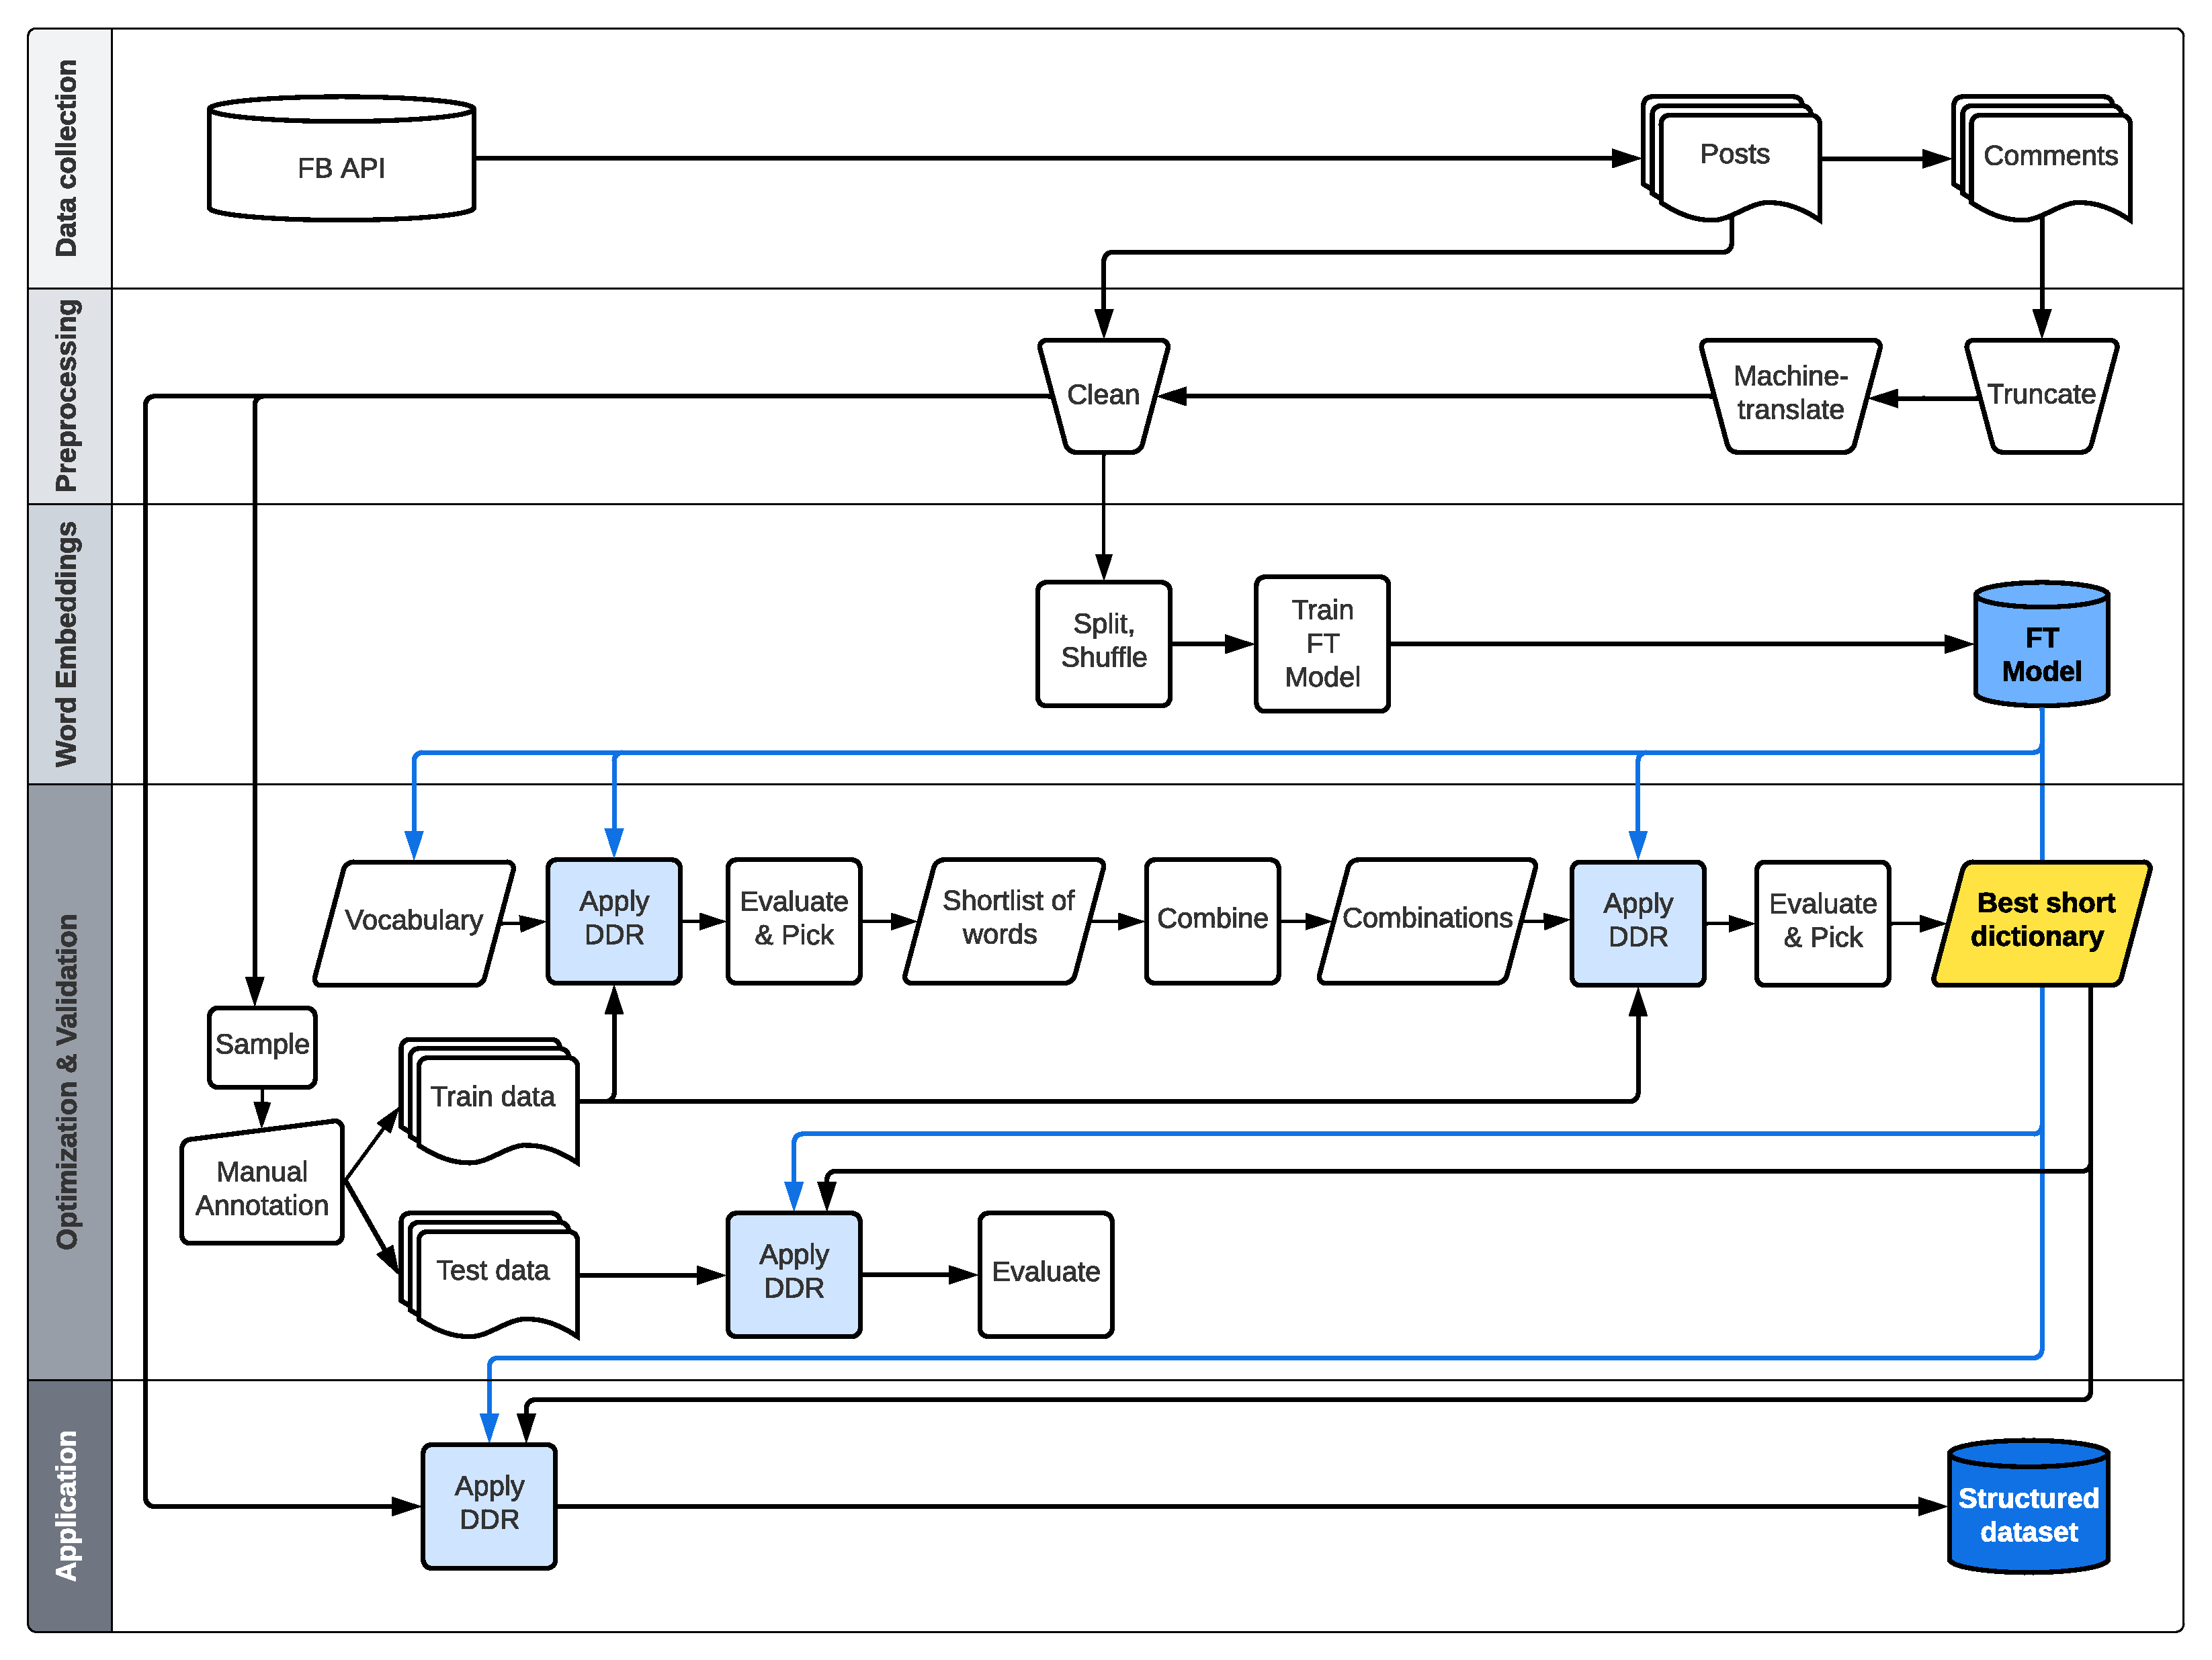
\includegraphics{plots/pipeline_CCR_paper_20230516.pdf}

}

\caption{Pipeline for Optimizing and Applying the DDR Measurement}

\end{figure}

\hypertarget{fasttext-model}{%
\subsubsection{\texorpdfstring{\emph{FastText}
Model}{FastText Model}}\label{fasttext-model}}

I trained a custom \emph{fastText} word embedding model (Bojanowski et
al. 2017) using the comprehensive corpus of German comments and
German-language posts, including translations. Word embeddings represent
the semantic relations between words in a multidimensional vector space
(Mikolov et al. 2013). These vector representations are produced by
machine learning algorithms trained on extensive text corpora. These
rely on the assumption that words of similar meaning repeatedly occur in
similar contexts (Mikolov et al. 2013). \emph{FastText} models,
distinguished from other embeddings, excel in handling social media
texts as they are robust against misspellings, can generate vectors for
out-of-vocabulary words, and perform well on morphologically rich
languages. These capabilities are achieved by segmenting words into
n-grams of characters, and inferring embeddings for these sub-word
snippets as well (Bojanowski et al. 2017).

For the task in this research, I preferred a custom-trained word
embedding model. Pre-trained, off-the-shelf models are typically sourced
from curated texts like Wikipedia, which lack authentic expressions of
populism. In addition, pre-trained models miss the meaning of terms with
current relevance. This seems particularly relevant in the context of
the COVID-19 crisis, which resulted in a whole vocabulary of new words.

The documents used for training underwent cleaning processes detailed in
Appendix B, were segmented into sentences using the \emph{quanteda}
(Benoit et al. 2018) tokenizer, and then randomized. After filtering
duplicates and sentences containing fewer than 5 words, the model
training dataset encompassed 3,564,352 lines of text.

The model was trained on a local machine (Intel(R) i7-8565U CPU @
1.80GHz, 4 cores, 8 threads, 16 GB RAM, no GPU) utilizing the
\emph{fastrtext} R-package (Benesty 2019). I chose the skipgram method
to train a model 200 dimensions, with the following hyperparameters: 20
epochs, learning rate .1, bucket size 2,000,000, context window size 7,
maximum n-gram length 6, minimum n-gram length 3, and set a minimum word
count threshold of 10 for inclusion in the vocabulary. The training
completed within less than 2 hours, yielding a vocabulary of 89,309
terms.

To evaluate the model's quality via face validity, I reviewed results
from several nearest neighbor queries using political terms. For the
formal validation, I focused on output validity, as reported in the main
article. The model, along with the replication materials, is included in
the replication repository: \url{https://osf.io/d4qng/}.

\hypertarget{optimizing-the-ddr-measurement}{%
\subsubsection{Optimizing the DDR
Measurement}\label{optimizing-the-ddr-measurement}}

The main article details the DDR method, validation data, and evaluation
strategy. This section focuses on outlining the steps taken to identify
an optimal DDR dictionary specifically geared toward capturing
user-generated expressions of populism. The objectives were threefold:
First, the dictionary should be \emph{inductively} derived, reflecting
genuine user-generated expressions of populism. At the same time,
second, the dictionary should be \emph{theory-driven}, reflecting core
dimensions of populism. Third, the resulting measurement should be
\emph{comparable}, maximizing F1 scores across all countries. The R-code
to replicate these steps is presented in the vignette `from text to
measurement' within my R-package \emph{dictvectoR} (Thiele 2022b). Due
to copyright restrictions, the original Facebook text data cannot be
shared. The data provided in the replication repository includes the
scores from applying the DDR measurement and shareable data.

Commencing with the 89,309 terms in the \emph{fastText} model's
vocabulary, I excluded the least common 10\% of words and stop-words.
Each word's cosine similarity to the average representation of two
corpora was computed: Firstly, to the average representation of all
comments tagged as populist in the training corpus and secondly, to the
representation of all non-populist comments in the training dataset.
Additionally, I computed the score difference, facilitated by
\texttt{dictvectoR::find\_distinctive()}. This initial process provided
rough indicators for words potentially enhancing the recall and
precision of the DDR score. I used the product of the populism
similarity and distinctiveness scores to narrow down the list of words
to 3,000 words. Multiword expressions frequently used in a random 50\%
subset of the corpus were added using
\texttt{dictvectoR::add\_multiwords()}. Multiword expressions are
important in populist communication, as they are used to construct in-
and out-groups (e.g., `wir steuerzahler') and distinguish neutral from
populist meanings of words. Next, F1 scores for each individual term
were obtained, by treating each term as one-term-dictionary in the DDR
and the annotated train sample for evaluation.
\texttt{dictvectoR::get\_many\_F1s()} takes care of this task. Highly
similar terms were dropped, keeping the best performing with
\texttt{dictvectoR::remove\_similar\_words()}.

Next, the words were reviewed manually. First, words were coarsely coded
for relevance. Highly idiosyncratic word combinations and
near-duplicates were dropped. Second, the remaining list of 287 terms
was annotated using a more nuanced classification. Terms were annotated
as referring to `elites', `the people', or some kind or `relation'
between those two antagonists. For `elites' I further annotated
subcategories. The terms annotated as `relation', contained the
subcategories `blaming', `manipulation', `sovereignty', `damaging', and
`unaccountable'. These categories were built inductively from the
identified words but reflect theoretical key dimension of populist
discourse. From each of the three dimensions, the 15 best performing
terms were selected.

Using combinatorics and random sampling, 2.9 million different
combinations of these 45 words were obtained. Dictionary lengths between
three to fifteen words were allowed, with at least one word per
dimension. The number of combinations was limited by randomly picking up
to 100 combinations for each number of words per dimension combination.
For example, instead of featuring all 3,003 combinations of length 5
from the 15 terms for `elites', only 100 were sampled and combined with
all combinations for the other dimensions.
\texttt{dictvectoR::get\_combis()} provides this function. The
performance of the DDR measurements for each of the 2.9 million
combinations was assessed by their F1 in predicting the human annotation
in the train data. For the 10k best-performing combinations, F1 scores
were computed additionally for each country. To evaluate consistency
across countries, the 8th root of the product of the overall F1 score
times all seven country F1 scores was calculated. The dictionary that
maximized F1 most consistently on the train data was selected. A manual
inspection, using the annotated subcategories, deemed that dictionary
conceptually balanced and convincing. This dictionary and the validation
results are documented in the main text.

\hypertarget{additional-equivalence-assessment}{%
\subsubsection{Additional Equivalence
Assessment}\label{additional-equivalence-assessment}}

In addition to the validation documented in the main text, I inspected
the importance of each single dictionary term for the measurement
performance across countries. To quantify the impact of each single
term, a list of 12 dictionaries was created where each dictionary left
out one of the 12 terms in the selected DDR dictionary. Each of these
`incomplete' dictionaries was used to predict populism in the (1)
combined test \& train validation sample, and (2) the test sample alone,
and a F1 score calculated, as described in the main article. To assess
deteriorated or improved performance, I inspect the difference between
the F1 scores for the `incomplete' and the complete DDR-dictionary. The
heat-map in Figure C2 documents how leaving out one of the 12
DDR-dictionary terms (y-axis) improves (positive values; light-yellow)
or deteriorates (negative values; dark-blue) the F1 score, compared to
the complete dictionary performance in predicting populism in the test
and train data (left grid) and test sample alone (right grid).

The performance of an ideal measurement would (a) not decrease strongly
by leaving out one term, (b) would exhibit a balanced pattern of term
importance, and (c) would exhibit similar patterns across all countries.
The heat-map in Figure C2 shows that the selected DDR-dictionary comes
close to achieving these goals for the untranslated Austrian and German
corpora: The differences there are relatively small
(\textless\textbar.03\textbar) and do not show outlying terms for both
the combined data, as well as the test data alone. Similarly homogeneous
patterns emerge for the Netherlands, and UK. The pattern is less
balanced for France, Sweden, and Italy. For example, leaving out the
term ``sogenannte experten'' decreases the performance on the French
train \& test corpus by -.05, and in likewise by -.05 in the Italian
test corpus. These patterns illustrate that country-contexts continue to
have an impact on the meaning of words, even after machine translation
(Licht and Lind 2023, 20), and hence affect measurement performance and
equivalence. The patterns are more imbalanced in the test data, which
seems concerning. However, it must be noted that these imbalances are
partly driven by the low number of true positives in the Italian (n= 22,
26\%) and Swedish (n=27; 32\%) test data, which is below the mean share
of true positives in population test dataset (40\%). As discussed in the
main article, the careful inspection of the DDR measurement raises
questions about its comparability across countries. Appendix E presents
a robustness check of the comparative findings resulting from the
regression analysis.

\begin{figure}

{\centering 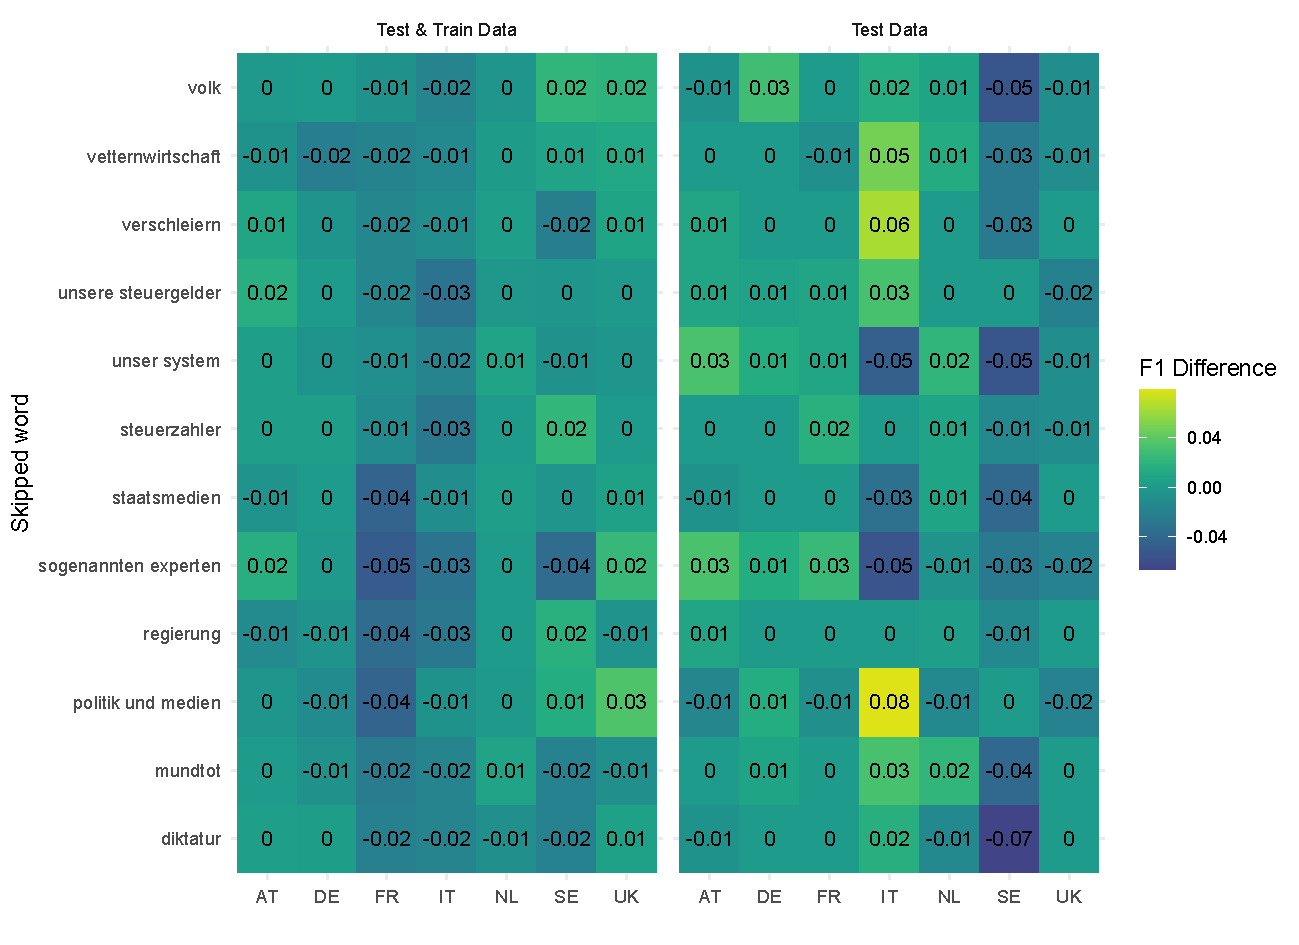
\includegraphics{plots/heatmap_skip_words_20231129.pdf}

}

\caption{Changes in F1 when leaving out single DDR-dictionary terms by
country}

\end{figure}

\newpage
\renewcommand{\thefigure}{D\arabic{figure}}
\renewcommand{\thetable}{D\arabic{table}}
\setcounter{figure}{0}
\setcounter{table}{0}

\hypertarget{appendix-d}{%
\subsection{Appendix D}\label{appendix-d}}

\hypertarget{dictionaries}{%
\subsubsection{Dictionaries}\label{dictionaries}}

The subsequent tables document the multilingual dictionaries used for
capturing references to \emph{COVID-19,} COVID-19 containment policies
(\emph{Measures),} lifting of restrictive policies (\emph{Easing)}, as
well as \emph{Experts} and the \emph{Government}. Notably, the
dictionaries for the first three categories share overlap, functioning
as sub-categories of one another: All terms within \emph{Measures} are
encompassed within \emph{COVID-19}, and all terms within \emph{Easing}
are included in \emph{Measures}.

The development of these dictionaries commenced with a manual
translation derived from an existing German dictionary (Thiele 2022a),
complemented by the utilization of translation websites (linguee.de;
context.reverso.net) providing contextualized translations. Each term's
suitability was determined through careful consideration of suggested
translations and contextual relevance. Ambiguous terms were excluded.
Subsequently, country-specific \emph{fastText} models were trained,
following the methodology detailed in Appendix C, utilizing the
non-translated post corpora. These models were employed to retrieve the
20 nearest neighbors for each term. The obtained results underwent a
secondary manual inspection, cross-referenced with context-sensitive
translation websites (linguee.de; context.reverso.net). Furthermore, I
used \texttt{quanteda::keywords-in-context()} to inspect the contextual
use of the identified keywords within the analyzed corpus. Both sources
of information were instrumental in supplementing the list of keywords,
increasing the precision of the dictionary, and inferring wildcard
placements.

The \emph{Government} dictionaries maintain case sensitivity and were
applied to the non-lowercased corpora. To enrich these dictionaries, I
compiled the names of the members of each country's national cabinets at
the time of analysis, occasionally excluding too common family names.
The German and Austrian dictionaries are identical except for their
\emph{Government} dictionary. All dictionaries are provided in a
machine-readable format in the replication repository.

{
\begin{spacing}{.9}
\fontsize{8}{9}\selectfont 
\begin{longtable}[]{@{}
  >{\raggedright\arraybackslash}p{.09\linewidth}
  >{\raggedright\arraybackslash}p{.12\linewidth}
  >{\raggedright\arraybackslash}p{.71\linewidth}@{}}
\caption{Dictionaries.} \\
\toprule\noalign{}
\textbf{Language} & \textbf{Concept} \newline \emph{(n words)} & \textbf{Words}\textsuperscript{a} \\
\midrule\noalign{}
\endhead
%\bottomrule\noalign{}
\endlastfoot 
\begin{minipage}[t]{\linewidth}\raggedright
DE\\
\strut \\
\strut
\end{minipage} & COVID-19 (124) & *ansteck*, *ausgangssperre*,
*cluster*, *geimpft*, *immunisier*, *impf*, *infektion*, *infizier*,
*lockdown*, *lockerung*, *maske*, *maskenpflicht, *maßnahme*, *pandemi*,
*quarantäne*, *reisebeschränkung*, *reiseverbot*, *schnelltest*,
*testpflicht*, *vakzin*, *viren*, *virus*, abstandsregel*, angesteckt*,
antigen*, antikörper*, arzneimittelbehörde, astra*,
ausgangsbeschränkung*, ausreisetestpflicht, biontech*, blutgerinnsel,
blutgerinnseln, bundesgesundheitsminister, corona*, cov, covid*, delta,
dosen, durchimpfung*, einreise*, einreisebeschränkung*,
einreisebestimmungen, einreisestop*, einreiseverbot*, epidemie*,
erkranken, erkrankung*, erreger, fallzahl*, ffp*, freitest*, gelockert,
genesungen, gesundheitsexperte, gesundheitsminister, gesundheitssystem*,
getestet*, ghebreyesus, gurgelt, herdenimmunität, home*office,
homeoffice*, hospitalisierungen, hygiene, hygieneregeln, impfpflicht,
intensivmedizinisch, intensivpatienten, intensivstationen, inzidenz*,
kontaktbeschränkungen, kontaktpersonen, kontaktverbot*, kontrollen,
körpernahe, lombardei, lungenkrankheit, masken*pflicht, massentest*,
mindestabstand, moderna, mutante, mutanten, mutation, mutationen,
neuinfektion*, notfallzulassung, öffnet, öffnungsschritt*, patienten,
pcr*, pfizer*, pharmaunternehmen, präsenzunterricht*, regeln,
reisewarnung*, reproduktionszahl*, risikogebiet*, risikogruppen, rki,
sars*, sauerstoff, schulöffnung*, schulschließung*, schutzmaske*,
schutzregel*, selbsttest*, social distanc*, sperrzone, spitalspatienten,
stark eingeschränkt, superspread*, tests, teststraße*, teststrategie*,
ungeimpft*, weiter eingeschränkt, weltgesundheitsorganisation, who,
wieler, wuhan, zeneca, zweite* welle \\ \cline{2-3}

& Measures (69)\textsuperscript{b} & *ausgangssperre*, *geimpft*,
*impf*, *lockdown*, *lockerung*, *maske*, *maskenpflicht, *maßnahme*,
*quarantäne*, *reisebeschränkung*, *reiseverbot*, *schnelltest*,
*testpflicht*, *vakzin*, abstandsregel*, antigen*, arzneimittelbehörde,
astra*, ausgangsbeschränkung*, ausreisetestpflicht, biontech*, dosen,
durchimpfung*, einreise*, einreisebeschränkung*, einreisebestimmungen,
einreisestop*, einreiseverbot*, ffp*, freitest*, gelockert, getestet*,
gurgelt, home*office, homeoffice*, hygiene, hygieneregeln, impfpflicht,
kontaktbeschränkungen, kontaktpersonen, kontaktverbot*, kontrollen,
masken*pflicht, massentest*, mindestabstand, moderna, notfallzulassung,
öffnet, öffnungsschritt*, pcr*, pfizer*, pharmaunternehmen, regeln,
reisewarnung*, risikogebiet*, schulöffnung*, schulschließung*,
schutzmaske*, schutzregel*, selbsttest*, social distanc*, sperrzone,
stark eingeschränkt, tests, teststraße*, teststrategie*, ungeimpft*,
weiter eingeschränkt, zeneca \\ \cline{2-3}

& Easing (5)\textsuperscript{c} & *lockerung*, gelockert, öffnet,
öffnungsschritt*, schulöffnung* \\ \cline{2-3}

& Experts (50) & *arzt, *ärzt*, *expert*, *forschen*, *forschende*,
*forscher*, *forschung*, *ologe, *ologen, *ologin, *professor*,
*spezialist*, *studie, *studien, *studiendaten*, *studienergebnis*,
*universität*, *wissenschaft*, anästhes*, apotheker, charité, drosten,
endokrinolog*, epidemiolog*, ethikrat*, fachleute*, fda, ghebreyesus,
immunolog*, impfkommission, infektiolog*, institut*, intensivmedizin,
intensivmediziner, johns hopkins, mediziner, meduni, mikrobiolog*,
pneumolog*, psycholog*, rki, robert koch, stiko, uni,
universitätsklinik*, vakzinolog*, virolog*, weltgesundheitsorganisation,
who, wieler \\ \cline{2-3}

& Government - AT (39)\textsuperscript{d} &
*inisterin Aschbacher, *kanzler*,
*koalition*, *minister*, *minister?, *ministerium*, *regierung*,
Anschober, Blümel, Brüssel, Christine Aschbacher, Edtstadler, EU
Kommission*, eu* Kommission*, Europäische* Kommission*, Faßmann,
Gewessler, Kabinett*, Kanzler*, Kocher, Kogler, Kommissionchefin,
Kommissionspräsidentin, Köstinger, Kurz, Lunacek, Magnus Brunner,
Minister, Ministerin, Ministerium*, Ministerrat*, Mückstein, Nehammer,
Raab, Regierung*, Schallenberg, Schramböck, Tanner, Zadic \\ \cline{2-3}

& Government - DE (38)\textsuperscript{d} &
*inisterin Schulze, *kanzler*, *koalition*,
*minister*, *minister?, *ministerium*, *regierung*, ?on der Leyen,
Altmaier, Barley, Brüssel, EU Kommission*, eu* Kommission*, Europäische*
Kommission*, Giffey, Heil, Helge Braun, Kabinett*, Kanzler*, Kanzleramt*
Braun, Karliczek, Klöckner, Kommissionchefin, Kommissionspräsidentin,
Kramp Karrenbauer, Lambrecht, Maas, Merkel*, Minister, Ministerin,
Ministerium*, Ministerrat*, Regierung*, Scheuer, Scholz, Seehofer,
Spahn, Svenja Schulze \\ \cline{1-3}

EN & COVID-19 (77) & *cluster*, *easing*, *hotspot*, *immuni*,
*infect*, *lockdown*, *pandemi*, *quarantine*, *vaccin*, *vaccinated*,
*vaxx*, *virus*, antibod*, astra*, ban family visit*, ban visit*,
biontech*, cases, combat coronavirus, contact tracing, containment
measure*, corona*, coronavirus measure*, coronavirus safety measure*,
coronavirus test*, covid measure*, covid test*, covid*, curfew,
distancing, dose*, doses, eases, easing, epidemic, epidemic measure*,
fatalit*, fight against covid, fight coronavirus, government response*,
health verification*, health* measure*, healthcare, isolat*, jab,
lifting, limit* travel*, major incident, mask*, mass test*, measure*
taken, measure* to combat, measure* to fight, moderna, outbreak, pcr*,
pfizer*, re?open*, reopening, restrictions, sanitiser, sars*, stem
spread, stem the spread, strict* measure*, superspread*, test and trace,
test positive, tested on covid, tested positive, testing, tougher
measure*, tracing app, transmission, travel ban*, travel restrictions,
wuhan \\ \cline{2-3}
& Measures (60)\textsuperscript{b} & *easing*, *immuni*, *lockdown*,
*quarantine*, *vaccin*, *vaccinated*, *vaxx*, astra*, ban family visit*,
ban visit*, biontech*, combat coronavirus, contact tracing, containment
measure*, coronavirus measure*, coronavirus safety measure*, coronavirus
test*, covid measure*, covid test*, curfew, distancing, dose*, doses,
eases, easing, epidemic measure*, fight against covid, fight
coronavirus, government response*, health verification*, health*
measure*, isolat*, jab, lifting, limit* travel*, major incident, mask*,
mass test*, measure* taken, measure* to combat, measure* to fight,
moderna, pcr*, pfizer*, re?open*, reopening, restrictions, sanitiser,
stem spread, stem the spread, strict* measure*, test and trace, test
positive, tested on covid, tested positive, testing, tougher measure*,
tracing app, travel ban*, travel restrictions \\ \cline{2-3}
& Easing (6)\textsuperscript{c} & *easing*, eases, easing, lifting,
re?open*, reopening \\ \cline{2-3}
& Experts (28) & doctor*, endocrinolog*, epidemiolog*, ethic* adviser,
expert*, extrapolate, fda, finds, ghebreyesus, health professional,
immunolog*, institute, johns hopkins, microbiolog*, pharmacists,
physician*, professor, psycholog*, public health england, pulmonolog*,
research*, scien*, specialist*, study, survey, technique, virolog*,
world health organi?ation \\ \cline{2-3}
& Government (48)\textsuperscript{d} & Alister Jack, Barclay, Ben
Wallace, Brandon Lewis, Braverman, Brussels, Buckland, Coffey,
commission president, Commission President, Dowden, EU commission*,
European commission, Eustice, Gove, government, Government, Hancock,
Hart, Jenrick, Johnson, Kwarteng, Liz Truss, Lord Frost, Mark Spencer,
Michael Ellis, Milling, minister, Minister, ministry, Ministry, of Bowes
Park, Patel, PM, prime minister Boris, Prime Minister Boris, Prime
Minister Johnson, Raab, Rees Mogg, secretary, Secretary, Shapps, Sharma,
Sunak, Trevelyan, UK prime minister, UK Prime Minister, Williamson \\ \cline{1-3}

FR & covid-19 (63) & *anticorps, *autotest*, *épidémie, *incidence,
*virus, antigéniques, astra*, biontech*, cas, cluster, confin,
confinement, confinements, contag*, contamin*, contre la *pandemie,
contre le *virus, contre le covid, corona*, couvre feu, cov, covid*,
décision* difficil*, déconfinement, doses, écol* ferm*, événements
annulés, fermés, fermeture*, ffp*, gestes barrières, hospitalisés,
immunis*, immunitaire, immunité, infect*, inocul*, masque*, mesures
barrières, mesures de confinement, mesures le covid, mesures
restrictives, moderna, nouvell* mesur*, pand*mie, pcr, pfizer*,
pharmaceutique, quarantaine, reconfinement, relâchement, réouverture,
restrictions, rouvert, sars*, stopcovid, télétravail*, test*,
transmission, vaccin*, variant, variants, wuhan \\ \cline{2-3}

& Measures (41) & *autotest*, antigéniques, astra*, biontech*, confin,
confinement, confinements, contre la *pandemie, contre le *virus, contre
le covid, couvre feu, décision* difficil*, déconfinement, doses, écol*
ferm*, événements annulés, fermés, fermeture*, ffp*, gestes barrières,
inocul*, masque*, mesures barrières, mesures de confinement, mesures le
covid, mesures restrictives, moderna, nouvell* mesur*, pcr, pfizer*,
pharmaceutique, quarantaine, reconfinement, relâchement, réouverture,
restrictions, rouvert, stopcovid, télétravail*, test*, vaccin* \\ \cline{2-3}

& Easing (4)\textsuperscript{c} & déconfinement, relâchement,
réouverture, rouvert \\ \cline{2-3}

& Experts (30) & *ologiste, *ologue, *ologues, chercheur*, conseil de la
santé, endocrinolog*, épidémiolog*, essai* clinique*, étude*, expert*,
fda, ghebreyesus, hcsp, immunolog*, infectiolo*, institut, johns
hopkins, médecin, médecins, microbiolog*, oms, organisation mondiale de
la santé, pneumolog*, professionnel* de santé, psycholog*, scien*,
spécialist*, traitement, université, virolog* \\ \cline{2-3}

& Government (40)\textsuperscript{d} & Bachelot, Belloubet, Blanquer,
Borne, Bruxelles, Buzyn, Castex, Collomb, Commission européenne,
Darmanin, Denormandie, Dupond-Moretti, Dupond Moretti, Edouard Philippe,
Flessel Colovic, Girardin, Gourault, gouvernement, Hulot, Le Drian, Le
Maire, Lecornu, Macron, Matignon, Mézard, ministère, ministre*,
Montchalin, Nyssen, Parly, Pénicaud, Pompili, président de la
République, président Emmanuel, président français, président Macron,
présidente de la Commission européenne, Travert, Véran, Vidal \\ \cline{1-3}

IT & COVID-19 (70) & *antigen*, *contag*, *epidemi*, *immun*,
*incidenz*, *infett*, *infez*, *pandemi*, *vaccin*, *vaccina*, *virale,
*virus*, allentament*, anti coronavirus, anti covid, anti virus,
anticorp*, astra zeneca, astrazeneca, biontech*, casi, contenere i*,
contenere la, contenimento, coprifuoco, coronavir*, cov, covid*,
decessi, delta, distanziamento, dosi, ffp*, guariti, impone, isolament*,
lockdown, lotta alla pandemia, mascherin*, misura, misure, misure
restrittive, misure rigide, morti, nuova stretta, passaporto sanitario,
pfizer, provvedimenti, quarantena, restrizioni, riaperture, riapre,
ricoverati, sars*, scuole chiuse, sintomi, superspreader, telelavor*,
test, trasmissibilità, trombosi, una stretta, variante, virologi,
virologia, wuhan, zona arancione, zona gialla, zona rossa, zone rosse \\ \cline{2-3}

& Measures (43)\textsuperscript{b} & *antigen*, *vaccin*, *vaccina*,
allentament*, anti coronavirus, anti covid, anti virus, astra zeneca,
astrazeneca, biontech*, contenere i*, contenere la, contenimento,
coprifuoco, distanziamento, dosi, ffp*, impone, isolament*, lockdown,
lotta alla pandemia, mascherin*, misura, misure, misure restrittive,
misure rigide, nuova stretta, passaporto sanitario, pfizer,
provvedimenti, quarantena, restrizioni, riaperture, riapre, scuole
chiuse, telelavor*, test, trombosi, una stretta, zona arancione, zona
gialla, zona rossa, zone rosse \\ \cline{2-3}
 
& Easing (3)\textsuperscript{c} & allentament*, riaperture, riapre \\ \cline{2-3}

& Experts (39) & agenzia italiana del farmaco, aifa, anestes*, autorità
sanitarie, borrelli, commissione sanitaria, dott, dottore*,
endocrinolog*, epidemiolog*, espert*, farmacisti, fda, fondazione,
ghebreyesus, immunolog*, infettivolog*, institut*, johns hopkins,
magrini, medici, medico, microbiolog*, oms, organizzazione mondiale
della sanità, pneumolog*, professore*, psicolog*, ricerc*, ricerca,
ricercatore, ricercatori, ricercatrice, scien*, specialist*, studi,
studio, università, virolog* \\ \cline{2-3}

& Government (59)\textsuperscript{d} & *inistro Bianchi, ?onsiglio dei
?inistri, ?residente del ?onsiglio, Amendola, Azzolina, Bellanova,
Boccia, Bonafede, Bonetti, Brunetta, Bruxelles, Carfagna, Cartabia,
Catalfo, Cingolani, Colao, commissione europea, Commissione europea,
Commissione Europea, Consiglio dei ministri, Conte, D'Incà, D Incà,
Dadone, Daniele Franco, De Micheli, Di Maio, Draghi, Fioramonti,
Fraccaro, Franceschini, Garavaglia, Garofoli, Gelmini, Giorgetti,
Giovannini, governo, Governo, Gualtieri, Guerini, Lamorgese, Manfredi,
Messa, minister?, Minister?, ministr?, Ministr?, Orlando, Patrizio
Bianchi, Patuanelli, Pisano, premier, presidente della ?ommissione
?uropea, presidente della ?ommissione Ue, Provenzano, Sergio Costa,
Spadafora, Speranza, Stefani \\ \cline{1-3}

NL & COVID-19 (110) & *antigeen*, *antilicham*, *besmet*, *inent*,
*infect*, *lockdown*, *masker*, *metermaatregel*, *pandemie*,
*quarantain*, *reisverbod*, *vaccin*, *virus*, afstand*,
anderhalvemetermaatschap*, anderhalvemeterregel,
anderhalvemetersamenlev*, astra*, avondklok*, avondklokken,
avondklokrellen, basisschool dicht, beperkende maatregel*, bezoekregel*,
bijwerkingen, biontech*, cluster*, code rood, corona, corona maatregel*,
corona*, coronabeleid, coronagevallen, coronamaatregelen, coronaregels,
coronatesten, coronatests, coronawet, covid*, doses, ema, epidemie*,
farmaceut, farmaceuten, ffp*, gaan dicht, gemuteerde,
geneesmiddelenbureau, geprikt, gevaccin*, gezondheidsraad,
gezondheidszorg*, groepsimmuniteit*, heropenen, injectie, inreisregel*,
kunnen open, maatregel*, maatregel* om de verspreiding, maatregel* tegen
het coronavirus, masker*, moderna, mondkapje*, mutatie, nieuwe
maatregel*, openingsplan, patiënten, pcr*, pfizer*, prikken, reisadvie*,
reisbeperk*, reisverbod*, reproductiegetal*, restaurants dicht,
risicogebied*, rivm, sars*, scholen dicht, sneltest*, sterfgevallen,
steunmaatregelen, strenge* maatregel*, terrassen open*, testen*,
teststrategie, teststraten, thuisblijven, thuiswerken, variant,
varianten, veiligheidsmaatregel*, verpleegafdelingen, verplicht,
versoepeld, versoepelen, versoepeling, versoepelingen,
virusmaatregelen*, voorlopig dicht, weer open*,
wereldgezondheidsorganisatie*, who, winkels dicht, wuhan, zelftest*,
ziekenhuis, ziekenhuisopnames, ziekenhuispersoneel, zorgsysteem* \\ \cline{2-3}

& Measures (58)\textsuperscript{b} & *antigeen*, *inent*, *lockdown*,
*masker*, *quarantain*, *reisverbod*, *vaccin*, afstand*,
anderhalvemeterregel, astra*, avondklok*, avondklokken, avondklokrellen,
bezoekregel*, biontech*, coronabeleid, coronamaatregelen, coronaregels,
coronatesten, coronatests, coronawet, doses, ema, farmaceut, ffp*,
geprikt, gevaccin*, heropenen, injectie, inreisregel*, kunnen open,
maatregel*, masker*, moderna, mondkapje*, openingsplan, pcr*, pfizer*,
prikken, reisadvie*, reisbeperk*, reisverbod*, risicogebied*, sneltest*,
steunmaatregelen, terrassen open*, testen*, teststrategie, teststraten,
thuiswerken, verplicht, versoepeld, versoepelen, versoepeling,
versoepelingen, virusmaatregelen*, weer open*, zelftest* \\ \cline{2-3}
 
& Easing (10)\textsuperscript{c} & heropenen, kunnen open,
openingsplan, steunmaatregelen, terrassen open*, versoepeld,
versoepelen, versoepeling, versoepelingen, weer open* \\ \cline{2-3}

& Experts (37) & *deskundige*, *expert*, *loog, *ologen, *onderzoek,
*onderzoek*, *onderzoeken, *onderzoeker*, *specialist*, *studie,
*studies, *wetenschap*, arts*, dokt?r*, epidemiolog*, fda, ggd,
ghebreyesus, hogeschool, hooglera*, immunolog*, istitut*, johns hopkins,
longarts*, microbiolog*, nvwa, planbureau*, professor*, psycholog*,
rijksinstituut, rivm, scp, studieresultaten, universiteit, virolog*,
wereldgezondheidsorganisatie, who \\ \cline{2-3}

& Government (46)\textsuperscript{d} & *inister Bruins, *inister
Schouten, *minister, *minister?, ?an Ark, ?an Engelshoven, ?an
Nieuwenhuizen, ?an Rijn, ?an Veldhoven, ?e Jonge, Barbara Visser,
Bijleveld, Blok, Bruno Bruins, Brussel, Carola Schouten,
Commissievoorzitter, de Bruijn, Europese Commissie, Grapperhaus, Henk
Kamp, Hoekstra, Kaag, kabinet*, Kabinet*, Knapen, Koolmees, Minister,
ministerie, Ministerie, ministerraad, Ollongren, overheid, Overheid,
premier, Premier, Raymond Knops, regering*, Regering*, Rutte, Sander
Dekker, Slob, van Nieuwenhuizen, van t Wout, Wiebes, Zijlstra \\ \cline{1-3}

SE & COVID-19 (110) & *epidemi*, *infekt*, *karantän*, *lockdown*,
*masker*, *pfizer*, *reseförbud*, *reserestriktion*, *vaccin*, *virus*,
antigen*, antikropp*, astra*, besöksförbud, biontech*, biverkningar,
blodproppar, bromsa* spridning*, corona strategi, corona*, coronaåret,
coronapandemin, coronarestriktioner*, coronasmittad, coronasmittade,
coronastrategi*, coronatest*, coronatider, covid strategi, covid test,
covid*, covidtest*, distansering, distansundervisning*, dödssiffran,
dosen, doserna, ema, farsot*, flockimmunitet*, folkhälsomyndighet*
rekommendation*, folkhälsomyndigheten, folkhälsomyndighetens,
folkhälsomyndighetens råd, folksamlingar, förblir stängt, fortsatt
stäng*, håll* avstånd, håll* hemma, håll* öppet, hålla gränser öppna,
hållas stängd, immunitet, immuniteten, incidens*, inreseförbud*,
inreserestriktion*, isoler*, kampen mot corona*, kampen mot covid*,
klartecken, kontaktförbud, läkemedelsbolaget, läkemedelsjätten,
lättnader, masstest*, modernas, munskydd*, mutation, mutationen,
nedstängning*, öpp* gräns*, öpp* igen, öppna, öppning*, pandemi*,
pandemilagen*, patienten, pcr*, restriktioner, restriktionerna,
riskområde*, sars*, självtest*, sjukhusen, sjukhusvård, sjukvård*,
skolorna öppnar, skolstängningar*, skyddsåtgärd*, smitt*, snabbtest*,
spridningen, stäng* alla, stäng* gräns*, stäng* sina gräns*, stäng*
skol*, stäng* sve*, stänga barer, stängd* krogarna, stängda, stoppa*
spridning*, testning*, testresultat, uppluckring, utegångsförbud*,
världshälsoorganisation*, wuhan, zeneca, zenecas \\ \cline{2-3}

& Measures (79)\textsuperscript{b} & *karantän*, *lockdown*, *masker*,
*pfizer*, *reseförbud*, *reserestriktion*, *vaccin*, antigen*, astra*,
besöksförbud, biontech*, biverkningar, blodproppar, bromsa* spridning*,
corona strategi, coronarestriktioner*, coronastrategi*, coronatest*,
covid strategi, covid test, covidtest*, distansering,
distansundervisning*, dosen, doserna, ema, folkhälsomyndighet*
rekommendation*, folkhälsomyndighetens råd, folksamlingar, förblir
stängt, fortsatt stäng*, håll* avstånd, håll* hemma, håll* öppet, hålla
gränser öppna, hållas stängd, inreseförbud*, inreserestriktion*,
isoler*, kampen mot corona*, kampen mot covid*, klartecken,
kontaktförbud, läkemedelsbolaget, läkemedelsjätten, lättnader,
masstest*, modernas, munskydd*, nedstängning*, öpp* gräns*, öpp* igen,
öppna, öppning*, pandemilagen*, pcr*, restriktioner, restriktionerna,
riskområde*, självtest*, skolorna öppnar, skolstängningar*,
skyddsåtgärd*, snabbtest*, stäng* alla, stäng* gräns*, stäng* sina
gräns*, stäng* skol*, stäng* sve*, stänga barer, stängd* krogarna,
stängda, stoppa* spridning*, testning*, testresultat, uppluckring,
utegångsförbud*, zeneca, zenecas \\ \cline{2-3}

& Easing (10)\textsuperscript{c} & håll* öppet, hålla gränser öppna,
klartecken, lättnader, öpp* gräns*, öpp* igen, öppna, öppning*, skolorna
öppnar, uppluckring \\ \cline{2-3}

& Experts (39) & *epidemiolog*, *expert*, *forskare, *forskaren,
*forskning*, *institutet, *läkare*, *läkarn*, *professor, *professorn,
*studie, *studier, *universitet*, *vetenskap*, fda, fhi, fhm,
folkhälsomyndighet*, forskarna, ghebreyesus, immunolog*, ivo, johns
hopkins, läkark*, mikrobiolog*, msb, psykolog*, sakkunnig*, scb,
sjukvårdsdirektör, socialstyrelsen, specialist*, statistiska
centralbyrån, tegnell, universitetssjukhuset, vaccinimmunolog*,
världshälsoorganisationen*, virolog*, who \\ \cline{2-3}

& Government (45)\textsuperscript{d} & *departement*, *minister,
*minister* Johansson, *minister?, Amanda Lind, Ann Linde, Anna Hallberg,
Baylan, Bolund, Bryssel, Damberg, Ekström, Eneroth, Ernkrans, EU
kommission*, Eva Nordmark, Fridh, Hans Dahlgren, Jennie Nilsson,
kommissionens ordförande, kommissionsordförande, Lena Hallengren,
Lindhagen, Löfven, Lövin, Magdalena Andersson, Margot Wallström, Micko,
Minister*, ministerrådet, Morgan Johansson, Peter Eriksson, Peter
Hultqvist, regering*, Regering*, regeringskansliet*, Regeringskansliet*,
Shekarabi, statsminister*, Statsminister*, statsråd*, Statsråd*,
Stenevi, Strandhäll, Ygeman \\ 
\midrule\noalign{}
\multicolumn{3}{@{}m{\textwidth}@{}}{\tiny{\emph{Notes:} : (a) A * represents a wildcard, it matches any number of characters or digits; (b) All terms included in ‘measures’ are also included in ‘COVID-19’; (c) All terms included in ‘easing’ are also included in ‘measures’ and ‘COVID-19’; (d) Case-sensitive.}}   \\
\end{longtable}
\end{spacing}
}

\newpage
\renewcommand{\thefigure}{E\arabic{figure}}
\renewcommand{\thetable}{E\arabic{table}}
\setcounter{figure}{0}
\setcounter{table}{0}

\newpage
\begin{landscape}

\hypertarget{appendix-e}{%
\subsection{Appendix E}\label{appendix-e}}

{
\begin{spacing}{.8}
\fontsize{7.5}{8}\selectfont 
\begin{longtable}[]{@{}
  >{\raggedright\arraybackslash}p{0.07\linewidth}
  >{\centering\arraybackslash}p{0.025\linewidth}
  >{\centering\arraybackslash}p{0.065\linewidth}
  >{\centering\arraybackslash}p{0.025\linewidth}
  >{\centering\arraybackslash}p{0.065\linewidth}
  >{\centering\arraybackslash}p{0.025\linewidth}
  >{\centering\arraybackslash}p{0.065\linewidth}
  >{\centering\arraybackslash}p{0.025\linewidth}
  >{\centering\arraybackslash}p{0.065\linewidth}
  >{\centering\arraybackslash}p{0.025\linewidth}
  >{\centering\arraybackslash}p{0.065\linewidth}
  >{\centering\arraybackslash}p{0.025\linewidth}
  >{\centering\arraybackslash}p{0.065\linewidth}
  >{\centering\arraybackslash}p{0.025\linewidth}
  >{\centering\arraybackslash}p{0.065\linewidth}@{}}
\caption{Bayesian linear regression models, non-pooled data.} \\
\toprule\noalign{}
\begin{minipage}[b]{\linewidth}\raggedright
\end{minipage} & 
\multicolumn{2}{p{0.115\linewidth}}{\centering
\textbf{AT}
} &
\multicolumn{2}{p{0.115\linewidth}}{\centering
\textbf{DE}
} &
\multicolumn{2}{p{0.115\linewidth}}{\centering
\textbf{FR}
} &
\multicolumn{2}{p{0.115\linewidth}}{\centering
\textbf{IT}
} &
\multicolumn{2}{p{0.115\linewidth}}{\centering
\textbf{NL}
} &
\multicolumn{2}{p{0.115\linewidth}}{\centering
\textbf{SE}
} &
\multicolumn{2}{p{0.115\linewidth}}{\centering
\textbf{UK}
}
\\
\emph{Predictors} & 
\multicolumn{1}{c}{\emph{Est.}} &
\multicolumn{1}{c}{\emph{CI (95\%)}} &
\multicolumn{1}{c}{\emph{Est.}} &
\multicolumn{1}{c}{\emph{CI (95\%)}} &
\multicolumn{1}{c}{\emph{Est.}} &
\multicolumn{1}{c}{\emph{CI (95\%)}} &
\multicolumn{1}{c}{\emph{Est.}} &
\multicolumn{1}{c}{\emph{CI (95\%)}} &
\multicolumn{1}{c}{\emph{Est.}} &
\multicolumn{1}{c}{\emph{CI (95\%)}} &
\multicolumn{1}{c}{\emph{Est.}} &
\multicolumn{1}{c}{\emph{CI (95\%)}} &
\multicolumn{1}{c}{\emph{Est.}} &
\multicolumn{1}{c}{\emph{CI (95\%)}} 
\\
\midrule\noalign{}
\endhead
%\bottomrule\noalign{}
\endlastfoot  
Intercept & -.03 &  -.07 -- .01 &   .08 & .05 -- .12    & .20   & .16 -- .24    & -.01  & -.06 -- .03 &     -.38 &  -.42 -- -.35 &  .11 & .07 -- .15 &  .03 & -.02 -- .07 \\
Comments count &    .10 &  .08 -- .12 & .18 & .17 -- .20    & .19   & .17 -- .21    & .17   & .15 -- .20    & .17   & .15 -- .18    & .06   & .04 -- .09    & .27   & .24 -- .29 \\
Days since outbreak &   -.04    & -.08 -- -.01  & .11   & .08 -- .15    & .01   & -.03 -- .05   & .05   & .01 -- .08    & -.00  & -.04 -- .03   & .05   & .02 -- .09    & -.07  & -.12 -- -.03 \\
First wave  & -.34  & -.40 -- -.27  & -.25  & -.32 -- -.18  & -.25  & -.33 -- -.17  & -.05  & -.13 -- .02   & -.17  & -.24 -- -.10  & -.19  & -.27 -- -.11  & -.09  & -.18 -- -.00 \\
Stringency \tiny(lagged)    & .02   & -.01 -- .05   & .00   & -.02 -- .03   & -.04  & -.07 -- -.02  & -.02  & -.05 -- .00   & .01   & -.02 -- .04   & -.03  & -.06 -- -.00  & .12   & .08 -- .16 \\
COVID-19 \tiny(mentioned) &     .17 & .13 -- .20    & .29   & .25 -- .32    & .09   & .05 -- .13    & .20   & .16 -- .24    & .30   & .26 -- .34    & .13   & .08 -- .17    & .21   & .16 -- .25 \\
Government \tiny(mentioned) & .56   & .51 -- .60    & .29   & .24 -- .33    & .47   & .41 -- .53    & .45   & .39 -- .51    & .59   & .54 -- .65    & .52   & .45 -- .58    & .58   & .51 -- .66 \\
Experts \tiny(mentioned)    & .13   & .07 -- .19    & .03   & -.02 -- .08   & .18   & .09 -- .26    & .07   & .01 -- .13    & .22   & .16 -- .27    & .15   & .10 -- .20    & .11   & .03 -- .19 \\
Media type \tiny(tabloid)   &  -.16 & -.20 -- -.12 &    -.70    & -.74 -- -.66  & -.54  & -.59 -- -.49  & -.40  & -.45 -- -.35  & .23   & .19 -- .27    & -.51  & -.56 -- -.46  & -.53  & -.59 -- -.48 \\
Media type \tiny(pub. broadcaster)  & .09   & .04 -- .15    & .25   & .21 -- .29    & -.13  & -.18 -- -.09  & .00   & -.05 -- .05   & .48   & .44 -- .53    & -.12  & -.17 -- -.07  & .08   & .02 -- .14 \\
Moderation  & .02   & -.06 -- .10   & -.17  & -.21 -- -.12  & -.14  & -.51 -- .22   & -.39  & -.94 -- .18   & -.22  & -.47 -- .03   & -.03  & -.14 -- .07   & -.22  & -.36 -- -.08 \\
Stringency x COVID-19   & .13   & .10 -- .17    & .10   & .07 -- .13    & .01   & -.03 -- .05   & .01   & -.04 -- .05   & .13   & .09 -- .16    & -.02  & -.06 -- .02   & -.01  & -.06 -- .04 \\
\midrule\noalign{}
Bayes R\textsuperscript{2} & 
\multicolumn{1}{l}{.13} & .12 -- .14 & 
\multicolumn{1}{l}{.34} & .33 -- .35 &
\multicolumn{1}{l}{.13} & .12 -- .14 &
\multicolumn{1}{l}{.12} & .11 -- .13 &
\multicolumn{1}{l}{.20} & .19 -- .22 &
\multicolumn{1}{l}{.09} & .08 -- .10 &
\multicolumn{1}{l}{.22} & .20 -- .23 \\
N   & 12,345 & &    10,066 & &  8,818 & &   8,547 & &   9,913   & &  9,123 & &  6,446 \\
\midrule\noalign{}
\multicolumn{14}{l}{\tiny{\emph{Notes:} Priors: intercept (normal 0, 10), b (normal 0, 10), $\sigma$ (Cauchy 0, .5). Bayes R\textsuperscript{2} estimated on 2,000 draws.}} \\
\end{longtable}
\end{spacing} 
}

\end{landscape}

As a robustness check for the comparative analysis presented in the main
article, Table E1 presents the outcomes of Bayesian regression models
fitted separately for each country, using non-pooled data. These models
encompass all variables featured in Model 3 of the main article,
excluding random effects on page level due to the limited categories
within the grouping variable, page, which comprises only 3 categories
per country. This is deemed insufficient even within a Bayesian
framework. While media type is included in these models, aligning with
the page variable when countries are examined independently, uncertainty
from the page level isn't directly modeled, resulting in narrower
credible intervals (CIs). Continuous variables in these models were
standardized and centered on country-means.

To corroborate the positive effect of stringency on populism when
mentioning COVID-19, as observed in Model 3 for Germany, Austria, and
the Netherlands in the main article, Figure E1 illustrates the populism
predictions under specified conditions from country-specific models.
Stringency ranges from the overall minimum (uniform across countries;
represented in yellow) to the overall maximum (depicted in purple). The
interaction of mentioning COVID-19 with this variable is set to 1, while
all other variables are set to 0 or their respective means, consistent
due to centering.

The distributions depict posterior draws, with lines indicating the 80\%
(bold) and 95\% (thin) CIs. The figure highlights substantial positive
effects of stringency on populism when COVID-19 is mentioned, observed
in the country samples of Austria, Germany, the Netherlands, and
additionally, the UK, supplementing the findings from the main article.
Conversely, these effects are either insignificant (Italy) or trend in
the opposite direction (FR, SE) in other countries. Inspecting the
Bayes-R\textsuperscript{2} in Table E1, which are estimated on 2,000
draws, shows that the fitted model explains an exceptionally large
variance (.34, {[}.33-.35{]}) in the German data. However, this does not
seem to be an artifact of language: Both, for the UK (.22,
{[}.20-.23{]}) and for the Netherlands (.20, {[}.19-.22{]}), we find
higher values of Bayes-R\textsuperscript{2} than for equally
German-speaking Austria (.13, {[}.12-.14{]}). Overall, although the CIs
might not fully capture the uncertainty from the page level, these
findings fortify the robustness of the country-specific effects
identified in Model 3 of the main article.

\begin{figure}

{\centering 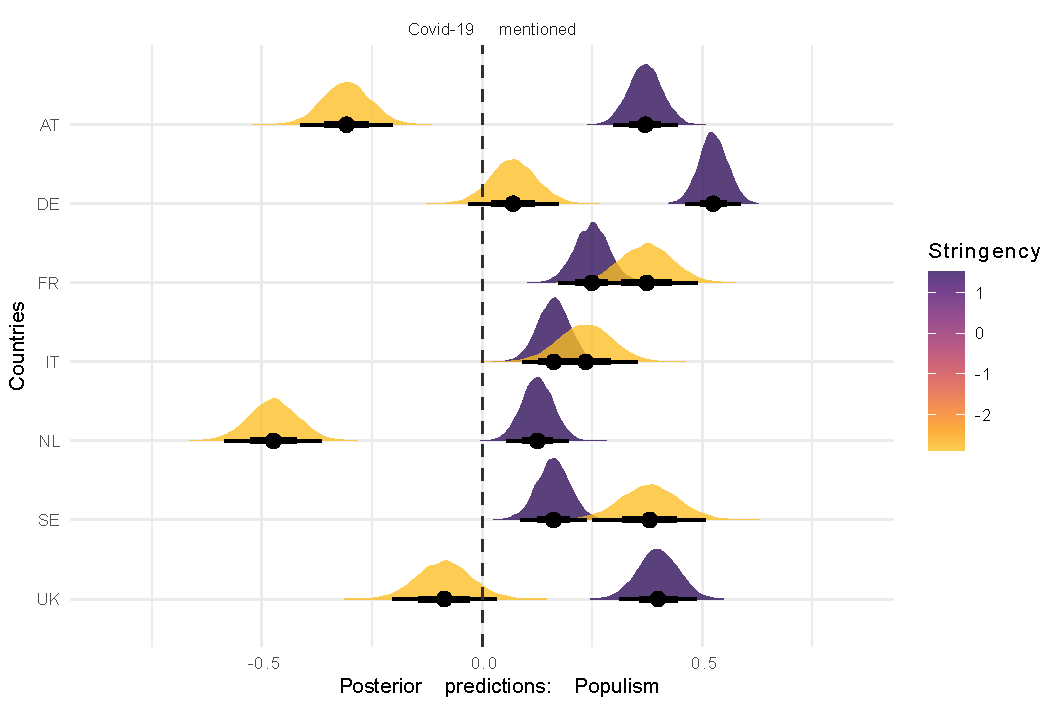
\includegraphics{plots/plot_strgXcov_SEP_ctry_fxdeff_20231130.pdf}

}

\caption{Conditional effects of stringency on the predicted level of
populism by country}

\end{figure}

\newpage

\hypertarget{references-in-the-appendix}{%
\subsection{References in the
Appendix}\label{references-in-the-appendix}}

\hypertarget{refs}{}
\begin{CSLReferences}{1}{0}
\leavevmode\vadjust pre{\hypertarget{ref-benesty2019Fastrtext}{}}%
Benesty, Michaël. 2019. {``Fastrtext 0.3.4.''}
\url{https://github.com/pommedeterresautee/fastrtext}.

\leavevmode\vadjust pre{\hypertarget{ref-benoit2018QuantedaPackage}{}}%
Benoit, Kenneth, Kohei Watanabe, Haiyan Wang, Paul Nulty, Adam Obeng,
Stefan Müller, and Akitaka Matsuo. 2018. {``Quanteda. {An R} Package for
the Quantitative Analysis of Textual Data.''} \emph{Journal of Open
Source Software} 3 (30): 774. \url{https://doi.org/10.21105/joss.00774}.

\leavevmode\vadjust pre{\hypertarget{ref-blassnig2019HittingNerve}{}}%
Blassnig, Sina, Sven Engesser, Nicole Ernst, and Frank Esser. 2019.
{``Hitting a Nerve: {Populist} News Articles Lead to More Frequent and
More Populist Reader Comments.''} \emph{Political Communication} 36 (4):
629--51. \url{https://doi.org/10.1080/10584609.2019.1637980}.

\leavevmode\vadjust pre{\hypertarget{ref-blassnig2016CodebookPopulist}{}}%
Blassnig, Sina, Sven Engesser, and Frank Esser. 2016. \emph{Codebook:
{Populist} Online Communication in {Europe}: {Self-presentation}, Media
Representation, and Audience Reconstruction of Political Actors}.
{Z{ü}rich}: {Courtesy by the Authors}.

\leavevmode\vadjust pre{\hypertarget{ref-bojanowski2017EnrichingWord}{}}%
Bojanowski, Piotr, Edouard Grave, Armand Joulin, and Tomas Mikolov.
2017. {``Enriching Word Vectors with Subword Information.''}
\emph{arXiv:1607.04606 {[}Cs{]}}, June.
\url{http://arxiv.org/abs/1607.04606}.

\leavevmode\vadjust pre{\hypertarget{ref-garten2018DictionariesDistributions}{}}%
Garten, Justin, Joe Hoover, Kate M. Johnson, Reihane Boghrati, Carol
Iskiwitch, and Morteza Dehghani. 2018. {``Dictionaries and
Distributions: {Combining} Expert Knowledge and Large Scale Textual Data
Content Analysis.''} \emph{Behavior Research Methods} 50 (1): 344--61.
\url{https://doi.org/10.3758/s13428-017-0875-9}.

\leavevmode\vadjust pre{\hypertarget{ref-licht2023GoingCrosslingual}{}}%
Licht, Hauke, and Fabienne Lind. 2023. {``Going Cross-Lingual: {A} Guide
to Multilingual Text Analysis.''} \emph{Computational Communication
Research} 5 (2): 1--31. \url{https://doi.org/10.5117/CCR2023.2.2.LICH}.

\leavevmode\vadjust pre{\hypertarget{ref-mikolov2013EfficientEstimation}{}}%
Mikolov, Tomas, Kai Chen, Greg Corrado, and Jeffrey Dean. 2013.
{``Efficient {Estimation} of {Word Representations} in {Vector
Space}.''} \emph{arXiv:1301.3781 {[}Cs{]}}, September.
\url{http://arxiv.org/abs/1301.3781}.

\leavevmode\vadjust pre{\hypertarget{ref-thiele2022PandemicPopulism}{}}%
Thiele, Daniel. 2022a. {``Pandemic Populism? {How Covid-19} Triggered
Populist {Facebook} User Comments in {Germany} and {Austria}.''}
\emph{Politics and Governance} 10 (1): 185--96.
\url{https://doi.org/10.17645/pag.v10i1.4712}.

\leavevmode\vadjust pre{\hypertarget{ref-thiele2022ThieledDictvectoR}{}}%
---------. 2022b. {``Thieled/{dictvectoR}.''}
\url{https://doi.org/10.5281/zenodo.7079600}.

\leavevmode\vadjust pre{\hypertarget{ref-thiele2022HowRightWing}{}}%
Thiele, Daniel, and Tjaša Turnšek. 2022. {``How {Right-Wing Populist
Comments Affect Online Deliberation} on {News Media Facebook Pages}.''}
\emph{Media and Communication} 10 (4): 141--54.
\url{https://doi.org/10.17645/mac.v10i4.5690}.

\end{CSLReferences}



\end{document}
